\documentclass{ieeeaccess}
\usepackage{cite}
\usepackage{amsmath,amssymb,amsfonts,amsthm,mathtools,bm}
\usepackage{algorithm}
\usepackage{algpseudocode}
\usepackage{graphicx}
\usepackage{textcomp}
\usepackage{booktabs,multirow,array}
\usepackage{siunitx}
\usepackage{enumitem}
\usepackage[nameinlink,noabbrev]{cleveref}
\usepackage{microtype}
\usepackage{url}

\graphicspath{{figures/}}
\newdimen\xfigwd
\xfigwd=\columnwidth
\def\BibTeX{{\rm B\kern-.05em{\sc i\kern-.025em b}\kern-.08em
    T\kern-.1667em\lower.7ex\hbox{E}\kern-.125emX}}

\newcommand{\M}{\mathbf{M}}
\newcommand{\K}{\mathbf{K}}
\newcommand{\C}{\mathbf{C}}
\newcommand{\A}{\mathbf{A}}
\newcommand{\Hq}{\mathbf{H}}
\newcommand{\I}{\mathbf{I}}
\newcommand{\PhiM}{\boldsymbol{\Phi}}
\newcommand{\ph}{\boldsymbol{\phi}}
\newcommand{\yy}{\mathbf{y}}
\newcommand{\uu}{\mathbf{u}}
\newcommand{\ff}{\mathbf{f}}
\newcommand{\rr}{\mathbf{r}}
\newcommand{\norm}[1]{\left\lVert #1\right\rVert}
\newcommand{\tr}{\operatorname{tr}}
\newcommand{\Var}{\operatorname{Var}}
\newcommand{\diag}{\operatorname{diag}}
\newcommand{\MAC}{\operatorname{MAC}}
\newcommand{\argmin}{\operatorname*{arg\,min}}
\newcommand{\argmax}{\operatorname*{arg\,max}}
\newtheorem{theorem}{Theorem}
\newtheorem{proposition}{Proposition}
\newtheorem{corollary}{Corollary}
\newtheorem{remark}{Remark}
\newtheorem{definition}{Definition}

\crefname{figure}{Fig.}{Figs.}
\Crefname{figure}{Fig.}{Figs.}
\crefname{table}{Table}{Tables}
\Crefname{table}{Table}{Tables}
\crefname{algorithm}{Algorithm}{Algorithms}
\Crefname{algorithm}{Algorithm}{Algorithms}
\crefname{section}{Section}{Sections}
\Crefname{section}{Section}{Sections}

\begin{document}
\history{}
\doi{}
\vol{7}
\year{2026}

\title{Qubits Are Not Enough: Deflation and Measurement Limits in Variational Quantum Modal Analysis}

\author{\uppercase{Bikalpa Gautam}\authorrefmark{1}, \uppercase{Akil Raj Subedi}\authorrefmark{2}}
\address[1]{Department of Civil, Environmental and Geomatic Engineering, ETH Zurich, 8093 Zurich, Switzerland}
\address[2]{Zynga Inc., Bangalore, India}

\markboth
{B. Gautam and A. R. Subedi: Qubits Are Not Enough: Deflation and Measurement Limits}
{B. Gautam and A. R. Subedi: Qubits Are Not Enough: Deflation and Measurement Limits}

\corresp{Corresponding author: Bikalpa Gautam (bgautam@ethz.ch)}

\begin{abstract}
Amplitude encoding stores an $N$-degree-of-freedom structural mode using $\lceil\log_2 N\rceil$ qubits, but compact encoding does not by itself make quantum modal analysis reliable or scalable. This article develops a rigorous evaluation framework for variational quantum eigensolvers applied to finite-element structural dynamics. A Cholesky transformation maps the generalized eigenproblem to a symmetric mass-orthonormal Hamiltonian, so Euclidean quantum-state orthogonality is identical to structural mass orthogonality. A two-scale normalization separates optimizer conditioning from spectrally safe padding. For higher modes, a necessary-and-sufficient deflation condition determines when the requested mode is the unique ground state, and a Davis--Kahan bound quantifies the effect of approximate lower-mode projectors. Numerical studies separate mapping correctness, ansatz expressibility, preprocessing, Pauli measurement growth, finite-shot frequency uncertainty, and damage localization. For structural chains with up to 128 degrees of freedom, consistent-mass whitening increases transformed-operator density from 0.023 to 0.308 and nonzero Pauli terms from 576 to 2950; a two- and three-dimensional generalization shows this densification worsens, and is delayed to larger problem sizes, as spatial dimension increases, and validates a subspace diagnostic against a genuine degenerate mode pair unreachable in one dimension. Exact state-vector experiments show that qubit count and circuit expressibility are distinct: shallow circuits fail even when the state dimension fits. At $10^5$ shots per Pauli term, the first-mode frequency root-mean-square error remains 2.23\%, while a 10\% stiffness loss is localized correctly in 26\% of trials. The results establish exact deflation conditions and engineering validation criteria, quantify major resource bottlenecks, and make no claim of quantum speedup.
\end{abstract}

\begin{keywords}
Finite-element eigenproblems, measurement complexity, structural dynamics, variational quantum eigensolvers.
\end{keywords}

\titlepgskip=-15pt
\maketitle

\section{Introduction}
\label{sec:intro}

\PARstart{M}{odal} analysis underlies seismic response, wind and pedestrian serviceability, reduced-order simulation, operational modal analysis, finite-element model updating, and vibration-based structural health monitoring \cite{Chopra2020,Ewins2000,FarrarWorden2012}. For a structure with $N$ unconstrained degrees of freedom (DOFs), the low-frequency modes solve
\begin{equation}
\K\ph_i=\lambda_i\M\ph_i,
\qquad \lambda_i=\omega_i^2,
\qquad f_i=\frac{\omega_i}{2\pi}.
\label{eq:gep}
\end{equation}
Classical Lanczos, subspace-iteration, and contour-based eigensolvers are mature and highly effective. A quantum method must therefore be evaluated against physical residuals, modal orthogonality, measurement cost, state-preparation cost, and end-to-end preprocessing, not against matrix dimension alone.

The variational quantum eigensolver (VQE) minimizes an expectation-valued Rayleigh quotient over a parameterized quantum state \cite{Peruzzo2014,McClean2016}. Excited-state extensions include variational quantum deflation (VQD) \cite{Higgott2019} and subspace-search VQE \cite{Nakanishi2019}. Generalized eigenvalue formulations have been developed for finite-element problems \cite{Sato2023}, and structural demonstrations have coupled finite-element software with VQE on simulators and small processors \cite{Liu2024}. More recently, Taliadouros et al.\ used SSVQE and VQD inside Monte Carlo simulation to estimate multiple eigenvalue statistics of stochastic structural systems, including a proof-of-concept execution on IBM Sherbrooke \cite{Taliadouros2025}. Accordingly, neither the classical Cholesky reduction nor the use of VQD/SSVQE for multiple structural eigenvalues is claimed as new here. The contribution relative to this literature is the exact deflation threshold, the approximate-projector perturbation analysis, the separation of padding certification from optimizer scaling, and end-to-end accounting of whitening, Pauli, finite-shot, and damage-decision costs. Existing studies establish feasibility, but do not by themselves establish scalable structural utility.

The central premise of this paper is summarized by its title: logarithmic qubit count is not sufficient. A usable structural modal solver must address six distinct questions:
\begin{enumerate}[label=(\roman*)]
\item Is the generalized eigenproblem mapped to a Hermitian operator without changing the physical mass metric?
\item Are padded and previously extracted states excluded with provable, rather than heuristic, penalty conditions?
\item Does whitening preserve or destroy sparsity and measurement economy?
\item Can the ansatz represent the requested eigenspace and can the cost be trained?
\item Can modal observables be estimated at finite-shot precision relevant to engineering decisions?
\item Can repeated monitoring distinguish genuine structural change from numerical mode swapping without biasing the eigensolution?
\end{enumerate}

The contributions are:
\begin{enumerate}[label=(\roman*)]
\item a mass-orthonormal Cholesky mapping and explicit accounting of its classical cost and sparsity consequences;
\item a two-scale spectral normalization that decouples optimizer scaling from certified safe padding;
\item an exact deflation theorem, a deterministic penalty-selection rule, and a perturbation bound for approximate projectors;
\item a lexicographic eigensolver that removes unjustified weighted sums of energy, variance, and leakage;
\item unbiased post-hoc temporal mode tracking based on uncertainty-normalized assignment, rather than continuity penalties in the eigensolver;
\item quantified Pauli, grouping, trainability, finite-shot, and damage-localization studies extending beyond a single three-qubit demonstration;
\item a two- and three-dimensional generalization showing that densification worsens, and is delayed to larger $N$, with spatial dimension, together with a degeneracy-diagnostic validation unreachable in one dimension.
\end{enumerate}

\Cref{fig:workflow} summarizes the end-to-end pipeline analyzed in the rest of the paper.

\begin{figure*}[t]
\centering
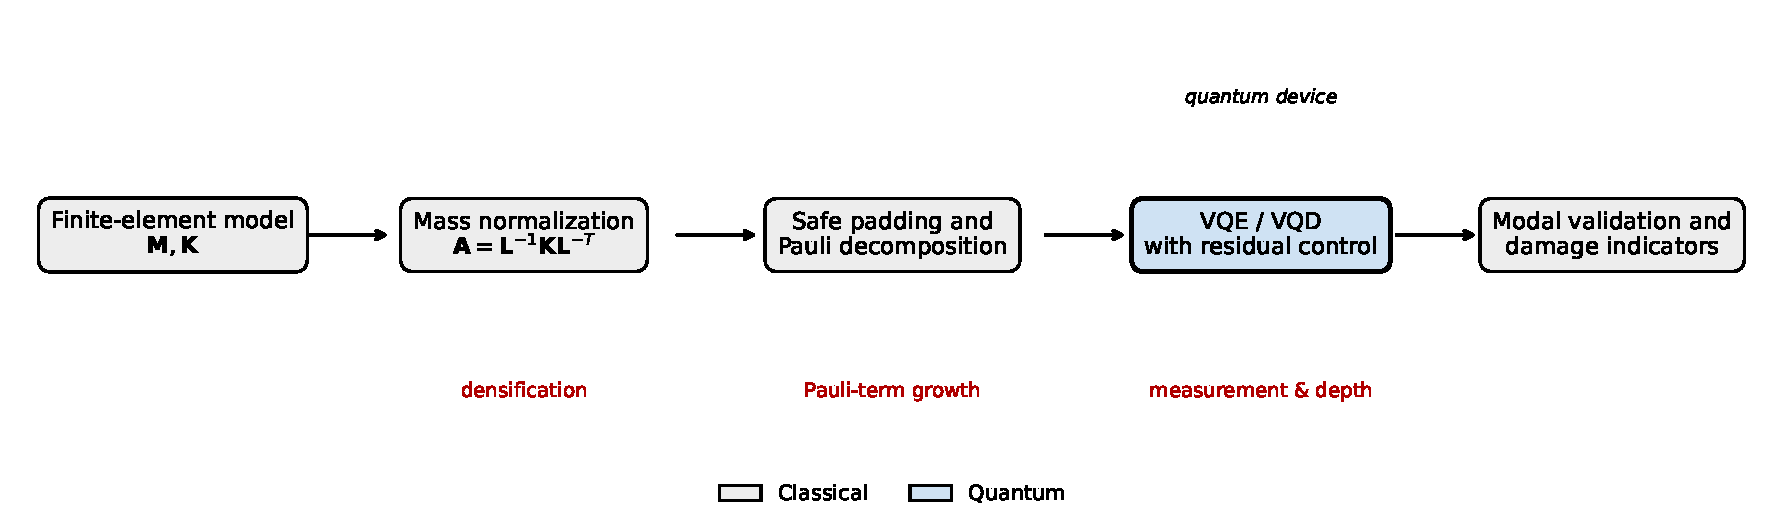
\includegraphics[width=\textwidth]{workflow.pdf}
\caption{End-to-end pipeline. A finite-element model $(\M,\K)$ is mass-normalized by the Cholesky map $\A=\mathbf L^{-1}\K\mathbf L^{-T}$, spectrally padded and Pauli-decomposed, solved by a variational eigensolver (VQE/VQD) with residual control, and finally converted into modal-validation and damage indicators. Each stage is analyzed for correctness, cost, and measurement precision separately. Red labels mark the dominant bottleneck stages; their asymptotic costs are quantified in \cref{tab:complexity}.}
\label{fig:workflow}
\end{figure*}

\section{Structural-dynamics foundation}
\label{sec:structural}

For a linear time-invariant structure,
\begin{equation}
\M\ddot{\uu}(t)+\C\dot{\uu}(t)+\K\uu(t)=\mathbf B_f\ff(t).
\label{eq:eom}
\end{equation}
Under uniform support acceleration $\ddot u_g(t)$,
\begin{equation}
\M\ddot{\uu}+\C\dot{\uu}+\K\uu=-\M\rr\ddot u_g(t).
\label{eq:base}
\end{equation}
For undamped free vibration, substitute $\uu(t)=\ph e^{\mathrm i\omega t}$ into \cref{eq:eom} to obtain \cref{eq:gep}. For a stable restrained structure, $\M$ and $\K$ are symmetric, $\M\succ0$, and the modes may be mass normalized:
\begin{align}
\PhiM_m^T\M\PhiM_m&=\I_m,\label{eq:massorth}\\
\PhiM_m^T\K\PhiM_m&=\boldsymbol\Omega_m^2,
\qquad \boldsymbol\Omega_m=\diag(\omega_1,\ldots,\omega_m).
\label{eq:stifforth}
\end{align}
The modal transformation $\uu=\PhiM_m\mathbf q$ yields, under classical damping,
\begin{equation}
\ddot{\mathbf q}+2\boldsymbol\Xi\boldsymbol\Omega_m\dot{\mathbf q}+\boldsymbol\Omega_m^2\mathbf q
=\PhiM_m^T\mathbf B_f\ff,
\label{eq:modal_eom}
\end{equation}
where $\boldsymbol\Xi=\diag(\xi_1,\ldots,\xi_m)$.

Finite-element assembly gives
\begin{equation}
\K=\sum_{e=1}^{n_e}\mathbf A_e^T\K_e\mathbf A_e,
\qquad
\M=\sum_{e=1}^{n_e}\mathbf A_e^T\M_e\mathbf A_e.
\label{eq:assembly}
\end{equation}
Boundary conditions are imposed before the quantum mapping. Penalty-enforced supports are avoided because artificial high stiffness can worsen conditioning and contaminate the spectrum.

\section{Mass-orthonormal Hermitian mapping and preprocessing}
\label{sec:mapping}

\subsection{Cholesky mapping}

The nonsymmetric product $\M^{-1}\K$ has the correct eigenvalues but is generally not Hermitian in the Euclidean metric. Let
\begin{equation}
\M=\mathbf L\mathbf L^T
\label{eq:chol}
\end{equation}
be a Cholesky factorization and define
\begin{equation}
\yy_i=\mathbf L^T\ph_i,
\qquad
\A=\mathbf L^{-1}\K\mathbf L^{-T}.
\label{eq:map}
\end{equation}
Then
\begin{equation}
\A\yy_i=\lambda_i\yy_i.
\label{eq:standard_eig}
\end{equation}

\begin{proposition}[Mass--Euclidean isometry]
If $\M\succ0$ and $\K=\K^T$, then $\A=\A^T$ and
\begin{equation}
\yy_i^T\yy_j=\ph_i^T\M\ph_j.
\label{eq:isometry}
\end{equation}
Thus Euclidean orthogonality of quantum states is exactly structural mass orthogonality after back-transformation.
\end{proposition}

\begin{proof}
Symmetry follows from $\A^T=\mathbf L^{-1}\K^T\mathbf L^{-T}=\A$. Moreover,
$\yy_i^T\yy_j=\ph_i^T\mathbf L\mathbf L^T\ph_j=\ph_i^T\M\ph_j$.
\end{proof}

The transformation should be implemented with triangular solves, not explicit inverses. Dense Cholesky has $O(N^3)$ arithmetic cost and $O(N^2)$ storage. Sparse cost depends on mesh dimension, ordering, and fill. For a class of two-dimensional finite-element meshes under nested dissection, Cholesky requires $O(N^{3/2})$ operations and $O(N\log N)$ nonzeros \cite{GeorgeNg1988}. These costs are classical preprocessing and must be included in any end-to-end comparison.

\subsection{Whitening can destroy locality}

Sparsity of $\M$ and $\K$ does not imply sparsity of $\A$. When $\M$ is diagonal, whitening is a diagonal scaling and often preserves graph locality. With a consistent mass matrix, $\mathbf L^{-1}$ can introduce long-range couplings. Define
\begin{equation}
\delta_A(\tau)=\frac{1}{N^2}\#\{(i,j):|A_{ij}|>\tau\norm{\A}_{\max}\}.
\label{eq:density}
\end{equation}
The transformed density $\delta_A$ is therefore an algorithmic observable, not a minor implementation detail.

A generalized Rayleigh quotient can avoid explicit whitening,
\begin{equation}
\mathcal R_G(\theta)=
\frac{\langle\psi(\theta)|\K|\psi(\theta)\rangle}
{\langle\psi(\theta)|\M|\psi(\theta)\rangle},
\label{eq:generalized_rq}
\end{equation}
as in generalized variational formulations \cite{Sato2023}. The trade-off is that both operators must be measured, the denominator must remain bounded away from zero, and higher-mode orthogonality must be enforced in the $\M$ metric. The Cholesky and generalized-quotient routes should therefore be compared rather than assuming that whitening is free.

\section{Two-scale spectral normalization and safe padding}
\label{sec:scaling}

\subsection{Two-scale normalization}

A Gershgorin upper bound is
\begin{equation}
U_G=\max_i\left(A_{ii}+\sum_{j\ne i}|A_{ij}|\right)
\ge\lambda_{\max}(\A).
\label{eq:gersh}
\end{equation}
Using $U_G$ as the sole scaling factor is safe but may compress the physical spectrum near zero. We therefore distinguish:
\begin{itemize}
\item an \emph{optimization scale} $s_t>0$, estimated for example by a short power or Lanczos iteration; and
\item the \emph{certified physical bound} $U=U_G/s_t$.
\end{itemize}
The optimization Hamiltonian is
\begin{equation}
\widetilde\A=\frac{\A}{s_t}.
\label{eq:tightscale}
\end{equation}
No assumption that $s_t\ge\lambda_{\max}$ is required.

\subsection{Spectral-safe padding}

Let $n_q=\lceil\log_2N\rceil$ and $D=2^{n_q}$. Define
\begin{equation}
\boxed{
\Hq_p=\begin{bmatrix}
\widetilde\A&\mathbf0\\
\mathbf0&\alpha\I_{D-N}
\end{bmatrix},
\qquad
\alpha=U+\delta_p,
\quad \delta_p>0.
}
\label{eq:safepad}
\end{equation}

\begin{proposition}[Safe padding under arbitrary positive scaling]
Every physical eigenvalue of $\widetilde\A$ is at most $U$, whereas every padded eigenvalue equals $U+\delta_p$. Hence padding cannot enter the physical low spectrum even when $s_t$ underestimates $\lambda_{\max}(\A)$.
\end{proposition}

\subsection{Effect of conservative scaling}

\begin{proposition}[Scalar-scaling law]
Let $\Hq_c=\Hq/c$ with $c>0$ and $E_c(\theta)=\langle\psi(\theta)|\Hq_c|\psi(\theta)\rangle$. Then eigenvectors and condition number are unchanged, while
\begin{equation}
\begin{aligned}
\lambda_i(\Hq_c)&=\lambda_i(\Hq)/c,\\
\nabla E_c&=\nabla E/c,\qquad
\Var_{\psi}(\Hq_c)=\Var_{\psi}(\Hq)/c^2.
\end{aligned}
\label{eq:scalinglaw}
\end{equation}
\end{proposition}

Consequently, excessive scaling does not change the exact eigenvectors, but it reduces absolute gaps and gradients and can interact badly with fixed optimizer tolerances and additive calibration errors. Under ideal shot noise, both signal and standard deviation scale as $1/c$, so relative precision is unchanged if all tolerances and coefficients are rescaled coherently. In practice, coherent rescaling requires the energy stopping tolerance, deflation margins, padding offset, confidence intervals, coefficient-pruning threshold, and any gradient threshold to be transformed by the same factor. The invariance fails when software retains fixed absolute tolerances, when coefficient truncation is not rescaled, or when hardware contributes an additive bias or noise floor that does not scale with the Hamiltonian coefficients. The optimization concern is therefore numerical and hardware-relative, not a universal loss of statistical information.

The physical frequency is recovered from $\widetilde\lambda_i$ by
\begin{equation}
f_i=\frac{1}{2\pi}\sqrt{s_t\widetilde\lambda_i}.
\label{eq:freqrecover}
\end{equation}

\section{Exact deflation conditions for multiple modes}
\label{sec:deflation}

\subsection{Ground-state VQE}

For a normalized parameterized state $|\psi(\theta)\rangle=U(\theta)|0\rangle^{\otimes n_q}$,
\begin{equation}
E(\theta)=\langle\psi(\theta)|\Hq_p|\psi(\theta)\rangle
\label{eq:vqe}
\end{equation}
upper-bounds the lowest eigenvalue accessible within the ansatz manifold. This is a variational statement, not a guarantee that a nonconvex classical optimizer finds the global minimum.

\subsection{Exact deflation theorem}

Let the non-padded eigenpairs of $\Hq_p$ be $(\varepsilon_k,|u_k\rangle)$ with
\begin{equation}
\varepsilon_1\le\varepsilon_2\le\cdots\le\varepsilon_N<\alpha.
\end{equation}
For target mode $r$, define the exact deflated operator
\begin{equation}
\Hq_r=\Hq_p+\sum_{j=1}^{r-1}\beta_jP_j,
\qquad P_j=|u_j\rangle\langle u_j|.
\label{eq:deflatedH}
\end{equation}

\begin{theorem}[Necessary and sufficient deflation threshold]
Assume $\varepsilon_r<\varepsilon_{r+1}$, with $\varepsilon_{N+1}:=\alpha$. Then $|u_r\rangle$ is the unique ground state of $\Hq_r$ if and only if
\begin{equation}
\boxed{\beta_j>\varepsilon_r-\varepsilon_j\quad\text{for all }j<r.}
\label{eq:betathreshold}
\end{equation}
\end{theorem}

\begin{proof}
The eigenvectors of $\Hq_r$ remain $|u_k\rangle$. For $k<r$, the corresponding eigenvalue is $\varepsilon_k+\beta_k$; for $k\ge r$, it is $\varepsilon_k$; padded states have eigenvalue $\alpha$. The target is the unique minimum precisely when every shifted lower eigenvalue exceeds $\varepsilon_r$ and $\varepsilon_{r+1},\alpha>\varepsilon_r$.
\end{proof}

The theorem replaces an arbitrary common penalty with a spectral condition. If a certified target upper bound $U_r\ge\varepsilon_r$ and prior eigenvalue error bounds $|\widehat\varepsilon_j-\varepsilon_j|\le\delta_j$ are available, a deterministic sufficient choice is
\begin{equation}
\boxed{
\beta_j=U_r-\widehat\varepsilon_j+\delta_j+\tau,
\qquad \tau>0.
}
\label{eq:certbeta}
\end{equation}
Indeed, $\varepsilon_j+\beta_j\ge U_r+\tau>\varepsilon_r$. Two bound policies are distinguished. A quantum-only spectral setup may use
\begin{equation}
U_r^{(G)}=U_G/s_t,
\label{eq:globalUr}
\end{equation}
which requires no auxiliary classical eigensolve but can be conservative. Alternatively, if $\vartheta_r^{(p)}$ is the $r$th Ritz value in a $p$-dimensional trial subspace, the min--max principle gives $\varepsilon_r\le\vartheta_r^{(p)}$; hence
\begin{equation}
U_r^{(R)}=\vartheta_r^{(p)}+\delta_{\mathrm{fp}}
\label{eq:ritzUr}
\end{equation}
is a tighter certified bound after allowing for floating-point error. A sparse $p$-step Lanczos/Ritz pass costs approximately $O(p\,\mathrm{nnz}(\A)+Np^2+p^3)$ arithmetic ($\mathrm{nnz}(\cdot)$ denoting the number of nonzero entries) and $O(Np)$ storage, and is therefore recorded explicitly as $C_{\mathrm{bound}}$ in the resource vector rather than treated as free preprocessing.

For a previously extracted mode, a practical high-confidence error radius can combine an eigenstate residual and Pauli-sampling uncertainty:
\begin{equation}
\begin{aligned}
\delta_j^{(\alpha_j)}&=\widehat r_j+
\sqrt{2\log(2/\alpha_j)\sum_{\ell}\frac{h_\ell^2}{n_\ell}},\\
\widehat r_j&=\norm{(\Hq_p-\widehat\varepsilon_j\I)|\widehat u_j\rangle}_2.
\end{aligned}
\label{eq:deltabound}
\end{equation}
The second term is a conservative Hoeffding radius for independent Pauli sampling. The residual locates the Rayleigh quotient near some eigenvalue; using it as a bound for mode $j$ additionally requires the estimated state to lie in the isolated modal interval assigned to $j$. In the exact threshold experiment below, exact eigenvalues are used only to verify theorem sharpness, so $\delta_j=0$; operational studies must report whether \cref{eq:globalUr} or \cref{eq:ritzUr} is used and include the corresponding classical cost.

\subsection{Approximate projectors and the cost of oversized penalties}

In practice, previous states are approximate. Let $\widehat P_j$ be the estimated projectors and
\begin{equation}
\widehat\Hq_r=\Hq_p+\sum_{j<r}\beta_j\widehat P_j,
\qquad
\Delta_r=\widehat\Hq_r-\Hq_r.
\label{eq:approxdefl}
\end{equation}
Then
\begin{equation}
\norm{\Delta_r}_2
\le\sum_{j<r}\beta_j\norm{\widehat P_j-P_j}_2.
\label{eq:deflperturb}
\end{equation}
Define the exact deflated separation
\begin{equation}
g_r=\min\left\{
\min_{j<r}(\varepsilon_j+\beta_j-\varepsilon_r),
\varepsilon_{r+1}-\varepsilon_r,
\alpha-\varepsilon_r
\right\}.
\label{eq:deflgap}
\end{equation}
If $\norm{\Delta_r}_2<g_r/2$, Weyl's inequality preserves an isolated target eigenvalue and the Davis--Kahan theorem gives the safe bound \cite{DavisKahan1970}
\begin{equation}
\boxed{
\sin\angle(\widehat u_r,u_r)
\le\frac{2\norm{\Delta_r}_2}{g_r}.
}
\label{eq:dkbound}
\end{equation}
Equation \eqref{eq:deflperturb} exposes the trade-off omitted by a heuristic penalty rule: a penalty must exceed the threshold, but an unnecessarily large penalty amplifies projector contamination. The recommended choice is therefore the smallest certified penalty satisfying \cref{eq:certbeta}, not indefinite adaptive growth.

\subsection{No arbitrary variance or leakage weights}

Hamiltonian variance remains a valuable residual:
\begin{equation}
\sigma_H^2(\psi)=\langle\Hq_p^2\rangle-\langle\Hq_p\rangle^2
=\norm{(\Hq_p-E\I)|\psi\rangle}_2^2.
\label{eq:variance}
\end{equation}
Padding leakage is
\begin{equation}
\ell_p(\psi)=\langle\psi|P_{\mathrm{pad}}|\psi\rangle.
\label{eq:leak}
\end{equation}
However, adding $\gamma\sigma_H^2+\zeta\ell_p$ to the energy creates uncalibrated trade-offs and changes the optimization landscape. The primary algorithm therefore uses only
\begin{equation}
C_r(\theta)=\langle\psi(\theta)|\widehat\Hq_r|\psi(\theta)\rangle.
\label{eq:primarycost}
\end{equation}
An optional lexicographic refinement is
\begin{equation}
\begin{aligned}
&\min_{\theta}\ \sigma_H^2(\theta)\\
&\text{s.t. }C_r(\theta)\le C_r^\star+\epsilon_E,\qquad
\ell_p(\theta)\le\epsilon_p,\\
&\hspace{2.0em}\max_{j<r}|\langle\widehat u_j|\psi(\theta)\rangle|^2\le\epsilon_O.
\end{aligned}
\label{eq:lexico}
\end{equation}
This preserves the energy ordering within a declared tolerance rather than hiding the trade-off in application-defined weights.

\begin{remark}[Scope of the guarantee]
Theorem 1 identifies the correct ground state of the full deflated Hilbert-space operator. It does not prove global convergence of a finite-depth ansatz or a nonconvex classical optimizer. Ansatz approximation error and optimization failure are measured separately through restarts, residuals, and depth studies.
\end{remark}

\subsection{Simultaneous and targeted alternatives}

SSVQE maps orthogonal input states through a common unitary, preserving orthogonality by construction \cite{Nakanishi2019}. For a target shift $\sigma$, the folded operator
\begin{equation}
\Hq_{\sigma}=(\Hq_p-\sigma\I)^2
\label{eq:folded}
\end{equation}
selects the mode nearest $\sigma$. These alternatives are useful when sequential projector error is unacceptable or when a narrow frequency band is known in advance.

\section{Trainability and ansatz expressibility}
\label{sec:trainability}

A real structural Hamiltonian permits a real-amplitude circuit,
\begin{equation}
U_L(\theta)=\prod_{\ell=1}^{L}
\left[U_{\mathrm{ent}}^{(\ell)}\prod_{q=1}^{n_q}R_y(\theta_{q\ell})\right]
\prod_{q=1}^{n_q}R_y(\theta_{q0}).
\label{eq:ansatz}
\end{equation}
Logarithmic qubit count does not imply shallow representability. A normalized real vector in $D=2^{n_q}$ dimensions has $D-1$ independent amplitudes, whereas a depth-$L$ hardware-efficient circuit has only $O(Ln_q)$ parameters. Therefore, a fixed-depth family cannot be universally expressive as $N$ grows.

Random parameterized circuits may exhibit barren plateaus in which gradient variance decays exponentially with qubit count \cite{McClean2018}. Cost-function locality can materially alter trainability, and even shallow circuits with global costs may exhibit barren plateaus \cite{CerezoBP2021}. Binary amplitude encoding and Cholesky whitening can turn a local structural operator into a nonlocal qubit Hamiltonian, so structural locality does not guarantee a local quantum cost. This concern is directly connected to the scaling results in \cref{sec:results}: for consistent mass, the transformed density grows to 0.308 and the Pauli count to 2950 at $N=128$, indicating that increasingly many computational-basis amplitudes and Pauli supports become coupled. Such densification moves the objective away from the local-cost setting in which trainability can be more favorable and toward the global-cost regime associated with gradient concentration. The present 2--12-qubit data cannot establish a structural barren plateau, but they show that whitening-induced nonlocality can worsen the locality condition as $N$ grows independently of whether circuit depth is increased. Quantifying this interaction for larger qubit counts, alternative orderings, and domain-decomposed mappings is therefore an open problem rather than an assumed asymptotic advantage.

For parameter $\theta_a$, the empirical trainability statistic used here is
\begin{equation}
V_g(n_q)=\Var_{\theta\sim\mathcal D}
\left[\frac{\partial E(\theta)}{\partial\theta_a}\right].
\label{eq:gradvar}
\end{equation}
A finite $n_q\le12$ study cannot prove or disprove an asymptotic barren plateau, but it can detect whether an exponential decay has already set in. Over the tested range it has not (\cref{sec:results}): the uniform-initialization gradient variance is better described by a polynomial than by an exponential in $n_q$, and its high-qubit slope is far shallower than an exponential collapse.

\section{Recovery, structural identification, and health-monitoring observables}
\label{sec:observables}

\subsection{Physical recovery and validation vector}

After removing padded coordinates, recover and mass-normalize
\begin{equation}
\ph_i=\mathbf L^{-T}\yy_i,
\qquad
\ph_i\leftarrow\frac{\ph_i}{\sqrt{\ph_i^T\M\ph_i}}.
\label{eq:recover}
\end{equation}
The normalized equilibrium residual is
\begin{equation}
\rho_i=
\frac{\norm{\K\ph_i^Q-\lambda_i^Q\M\ph_i^Q}_2}
{\norm{\K\ph_i^Q}_2+|\lambda_i^Q|\norm{\M\ph_i^Q}_2}.
\label{eq:residual}
\end{equation}
Multi-mode errors are
\begin{align}
\epsilon_M&=\norm{(\PhiM^Q)^T\M\PhiM^Q-\I}_F,\label{eq:em}\\
\epsilon_K&=\frac{\norm{(\PhiM^Q)^T\K\PhiM^Q-(\boldsymbol\Omega^Q)^2}_F}
{\norm{(\boldsymbol\Omega^Q)^2}_F}.\label{eq:ek}
\end{align}
No scalar exponential integrity index is introduced. Instead, every mode is reported through the non-aggregated diagnostic vector
\begin{equation}
\boxed{
\mathcal D_i=
(\epsilon_{f,i},\rho_i,\sigma_{H,i}^2,\ell_{p,i},o_i,1-\MAC_{ii}^{(M)}),
}
\label{eq:diagnosticvector}
\end{equation}
where $o_i=\max_{j<i}|\langle\widehat u_j|\widehat u_i\rangle|^2$. Acceptance thresholds are application-specific and must be stated component by component.

The mass-weighted modal assurance criterion is \cite{Allemang1982}
\begin{equation}
\MAC_{ij}^{(M)}=
\frac{|(\ph_i^C)^T\M\ph_j^Q|^2}
{[(\ph_i^C)^T\M\ph_i^C][(\ph_j^Q)^T\M\ph_j^Q]}.
\label{eq:mac}
\end{equation}
For a near-degenerate group, compare invariant subspaces. If
\begin{equation}
(\mathbf Y_C)^T\mathbf Y_Q=\mathbf U\cos\boldsymbol\Theta\mathbf V^T,
\end{equation}
then
\begin{equation}
\epsilon_{\mathrm{sub}}=\norm{\sin\boldsymbol\Theta}_F
\label{eq:subspace}
\end{equation}
is invariant to rotations inside the repeated eigenspace.

\subsection{Participation and frequency response}

For base excitation,
\begin{equation}
\Gamma_i=\frac{\ph_i^T\M\rr}{\ph_i^T\M\ph_i},
\qquad M_i^*=\Gamma_i^2
\label{eq:participation}
\end{equation}
for mass-normalized modes. The truncated modal frequency-response function is
\begin{equation}
\Hq_m(\omega)=\sum_{i=1}^{m}
\frac{\ph_i\ph_i^T}
{\omega_i^2-\omega^2+2\mathrm i\xi_i\omega_i\omega}.
\label{eq:frf}
\end{equation}
Frequency accuracy without participation, shape, and response accuracy is not sufficient for structural use.

\subsection{Connection to output-only identification}

For measured output power spectral density,
\begin{equation}
\mathbf S_{yy}(\omega)=\mathbf U(\omega)\boldsymbol\Sigma(\omega)\mathbf U^H(\omega),
\label{eq:fdd}
\end{equation}
and the dominant singular vector near resonance approximates the measured mode shape under the assumptions of frequency-domain decomposition \cite{Brincker2001}. Stochastic subspace identification uses
\begin{equation}
\mathbf x_{k+1}=\mathbf A_d\mathbf x_k+\mathbf w_k,
\qquad
\mathbf y_k=\mathbf C_d\mathbf x_k+\mathbf v_k,
\label{eq:ssi}
\end{equation}
with continuous poles $s_i=\log\mu_i/\Delta t$, frequencies $f_i=|s_i|/(2\pi)$, and damping ratios $\xi_i=-\Re(s_i)/|s_i|$ \cite{Peeters1999,Peeters2001,Reynders2012}. Experimental covariance estimates may define uncertainty-weighted MAC through $\mathbf W_i=\boldsymbol\Sigma_{\phi_i}^{-1}$ \cite{Reynders2008}.

\subsection{Unbiased temporal mode tracking}

Every monitoring epoch is solved independently using the same independently defined objective. A previous solution may initialize the circuit, but it does not enter the objective. After solution, define for candidate pair $(i,j)$
\begin{equation}
\mathbf z_{ij,t}=
\begin{bmatrix}
\log(f_{j,t}/f_{i,t-1})\\
1-\MAC_{ij,t}^{(M)}
\end{bmatrix},
\qquad
c_{ij,t}=\mathbf z_{ij,t}^T\boldsymbol\Sigma_{i,0}^{-1}\mathbf z_{ij,t},
\label{eq:trackingcost}
\end{equation}
where $\boldsymbol\Sigma_{i,0}$ is estimated from healthy baseline variability. Mode labels are assigned by
\begin{equation}
\pi_t^*=\argmin_{\pi}\sum_i c_{i,\pi(i),t}.
\label{eq:hungarian}
\end{equation}
A change alarm is based on $c_{i,\pi(i),t}$ exceeding a baseline quantile or a calibrated $\chi^2$ threshold. Because pairing occurs after independent eigensolution, it cannot pull a damaged mode toward its healthy predecessor. Near degeneracy, the same procedure is applied to principal angles between subspaces.

\subsection{Sensor-space recovery}

For sensor selector $\mathbf c_s$,
\begin{equation}
\phi_{i,s}=\mathbf c_s^T\ph_i
=\mathbf c_s^T\mathbf L^{-T}\yy_i
=\mathbf d_s^T\yy_i,
\qquad \mathbf d_s=\mathbf L^{-1}\mathbf c_s.
\label{eq:sensor}
\end{equation}
Therefore
\begin{equation}
\phi_{i,s}=\norm{\mathbf d_s}_2\langle\widehat d_s|\psi_i\rangle.
\label{eq:sensoroverlap}
\end{equation}
This can reduce readout when only instrumented coordinates are needed, although preparing $|\widehat d_s\rangle$ has its own cost. It is resource-favorable only when $\mathbf d_s=\mathbf L^{-1}\mathbf c_s$ has exploitable sparsity, low-rank structure, or a reusable preparation oracle; if whitening makes $\mathbf d_s$ dense and unstructured, generic amplitude preparation can require $O(N)$ gates and may erase the advantage over recovering the required classical amplitudes directly.

\subsection{Damage sensitivity and modal strain energy}

Let element damage reduce stiffness:
\begin{equation}
\K(\mathbf d)=\sum_{e=1}^{n_e}(1-d_e)\mathbf A_e^T\K_e^0\mathbf A_e.
\label{eq:damageK}
\end{equation}
For mass-normalized modes and stiffness-only damage,
\begin{equation}
\frac{\partial\lambda_i}{\partial d_e}
=-\ph_i^T\K_e^0\ph_i.
\label{eq:sensitivity}
\end{equation}
The element modal-strain-energy fraction is
\begin{equation}
\eta_{e,i}=
\frac{\ph_i^T\K_e\ph_i}{\ph_i^T\K\ph_i}.
\label{eq:mse}
\end{equation}
With
\begin{equation}
\Hq_e=\frac{\mathbf L^{-1}\K_e\mathbf L^{-T}}{s_t},
\label{eq:He}
\end{equation}
one obtains
\begin{equation}
\eta_{e,i}=
\frac{\langle\psi_i|\Hq_e|\psi_i\rangle}
{\langle\psi_i|\widetilde\A|\psi_i\rangle}.
\label{eq:qmse}
\end{equation}
A multimode change score is
\begin{equation}
D_e=\sum_{i=1}^{m}w_i|\eta_{e,i}^{d}-\eta_{e,i}^{0}|,
\qquad \sum_iw_i=1.
\label{eq:damageindex}
\end{equation}
This class of energy-based localization is related to established modal strain-energy methods \cite{Stubbs1995,Cornwell1999}. The finite-shot study below tests whether the quantum expectation formulation remains usable when the exact modes are no longer assumed available.

\section{Measurement and resource accounting}
\label{sec:resources}

\subsection{Pauli representation}

For $n_q$ qubits,
\begin{equation}
\Hq=\sum_{\ell=1}^{N_P}h_\ell P_\ell,
\qquad P_\ell\in\{I,X,Y,Z\}^{\otimes n_q},
\label{eq:pauli}
\end{equation}
where
\begin{equation}
h_\ell=2^{-n_q}\tr(P_\ell\Hq).
\end{equation}
Since $4^{n_q}\le4N^2$, the worst-case Pauli basis grows quadratically in the encoded structural dimension. Actual nonzero count depends on ordering, padding, mass model, and whitening. Commuting-group methods can reduce circuit settings but not eliminate finite-sampling error \cite{Crawford2021}.

Arbitrary amplitude-state preparation may itself require gate counts exponential in qubit number in the worst case, despite logarithmic qubit storage \cite{PleschBrukner2011}. Resource reports must therefore include state preparation, two-qubit gates, circuit depth, Pauli terms, commuting groups, shots, and optimizer evaluations.

\subsection{Finite-shot propagation}

For an independently measured Pauli mean $\mu_\ell$ with $n_\ell$ shots,
\begin{equation}
\Var(\widehat\mu_\ell)=\frac{1-\mu_\ell^2}{n_\ell}.
\label{eq:paulivar}
\end{equation}
Ignoring covariance between groups,
\begin{equation}
\Var(\widehat E)=\sum_\ell h_\ell^2\frac{1-\mu_\ell^2}{n_\ell}.
\label{eq:energyvar}
\end{equation}
For fixed total shots, the continuous optimal allocation satisfies
\begin{equation}
n_\ell\propto |h_\ell|\sqrt{1-\mu_\ell^2}.
\label{eq:allocation}
\end{equation}
The delta method gives
\begin{equation}
\Var(\widehat f_i)\approx
\left(\frac{s_t}{8\pi^2f_i}\right)^2\Var(\widehat\varepsilon_i).
\label{eq:freqvar}
\end{equation}
The $1/f_i^2$ factor makes the fundamental frequency especially vulnerable when its eigenvalue is small compared with the total Pauli-estimator variance.

\subsection{Controlled error budget}

An additive scalar ``total error'' is generally not identifiable because the components interact. We report the controlled error vector
\begin{equation}
\mathcal E=
(\epsilon_{\mathrm{FE}},\epsilon_{\mathrm{map}},\epsilon_{\mathrm{ansatz}},
\epsilon_{\mathrm{opt}},\epsilon_{\mathrm{shot}},\epsilon_{\mathrm{channel}},
\epsilon_{\mathrm{readout}}).
\label{eq:errorvector}
\end{equation}
In this paper, mapping error is zero up to floating-point arithmetic; ansatz and optimizer error are separated using exact state vectors and multiple restarts; shot error is evaluated by Monte Carlo sampling; and a stylized channel/readout sensitivity is reported only as a diagnostic. Finite-element modelling error and real-device error remain unquantified and are explicitly excluded from claims.

No dimensionally mixed ``information efficiency'' is defined. Instead, the raw resource vector is reported:
\begin{equation}
\begin{aligned}
\mathcal R=(&n_q,N_P,N_G,N_{\mathrm{shot}},N_{\mathrm{eval}},D_{\mathrm{circ}},N_{2q},\\
&C_{\mathrm{asm}},C_{\mathrm{chol}},C_{\mathrm{bound}},C_{\mathrm{Pauli}},C_{\mathrm{prep}}).
\end{aligned}
\label{eq:resourcevector}
\end{equation}
where $N_G$ is the number of measurement groups; $C_{\mathrm{asm}}$, $C_{\mathrm{chol}}$, $C_{\mathrm{bound}}$, and $C_{\mathrm{Pauli}}$ denote classical matrix assembly, whitening, spectral-bound, and Pauli-construction costs; and $C_{\mathrm{prep}}$ is quantum state-preparation cost. When the global Gershgorin policy \cref{eq:globalUr} is used, $C_{\mathrm{bound}}$ contains only the row-sum calculation. When a Ritz/Lanczos bound is used, its iterations, matrix--vector products, storage, and projected eigensolve are reported explicitly.

\subsection{End-to-end asymptotic cost}
\label{sec:complexity}

The resource vector \cref{eq:resourcevector} collapses into asymptotic order for the tested one-dimensional chains, where $\M$ and $\K$ are banded with constant half-bandwidth $b$. In the following, $k$ is the number of requested modes, $N_P$ the number of nonzero Pauli terms \eqref{eq:pauli}, $N_{\mathrm{eval}}$ the number of optimizer evaluations, $T_{\mathrm{it}}$ the classical Lanczos iteration count, and $\varepsilon$ the target accuracy of a single energy estimate. \Cref{tab:complexity} compares a sparse classical eigensolver with the variational quantum pipeline for the $k$ lowest modes of an $N$-DOF chain.

\begin{table}[t]
\centering
\caption{End-to-end asymptotic time and space for the $k$ lowest modes of an $N$-DOF banded 1D chain (constant half-bandwidth $b$). Dashes mark steps the classical solver does not perform.$^{\ddagger}$}
\label{tab:complexity}
\begin{tabular}{lll}
\toprule
Stage & Classical (Lanczos) & Quantum (VQD)\\
\midrule
Assembly & $O(N)$ & $O(N)$\\
Cholesky of $\M$ & --- & $O(Nb^2)=O(N)$\\
Whitening $\A$ & --- & $O(N^2)$\\
Pauli decomposition & --- & $O(N^2\log N)$\\
Solve / measure & $O(kN\,T_{\mathrm{it}})$ & $O(kN^2\varepsilon^{-2}N_{\mathrm{eval}})$\\
\midrule
Total time & $O(kN\,T_{\mathrm{it}})$ & $O(kN^2\varepsilon^{-2}N_{\mathrm{eval}})$\\
Space & $O(Nk)$ & $O(N)+O(N^2)^{\dagger}$\\
\bottomrule
\end{tabular}

\vspace{0.35em}
\parbox{\columnwidth}{\footnotesize $T_{\mathrm{it}}$ is the Lanczos iteration count: approximately constant with shift-invert ARPACK, and $O(\sqrt N)$--$O(N)$ for unpreconditioned Lanczos depending on the relative spectral gap. $^{\dagger}$$O(N)$ statevector amplitudes plus $O(N^2)$ classical storage for the dense-whitened operator and its Pauli list. $^{\ddagger}$Spectral-safe padding costs $O(D-N)=O(N)$ since $D<2N$, and the cheap (Gershgorin) bound policy costs $O(N^2)$; both are dominated by the whitening row above and are therefore omitted. The optional tighter Ritz/Lanczos bound policy \eqref{eq:ritzUr} instead costs $O(p\,\mathrm{nnz}(\A)+Np^2+p^3)$ time and $O(Np)$ space, a genuine additional cost not always dominated by whitening, reported separately as $C_{\mathrm{bound}}$.}
\end{table}

Three consequences follow. First, preprocessing is not the bottleneck for these chains: the banded Cholesky is $O(N)$, not the $O(N^3)$ dense cost noted in \cref{sec:mapping}. Second, the classical solver acts on the sparse $\K$ directly, so its cost scales with $\mathrm{nnz}(\K)=O(N)$, whereas whitening densifies $\A$---from density $0.023$ to $0.308$ between lumped and consistent mass at $N=128$---so the Pauli representation carries $N_P=O(N^2)$ terms in the worst case ($4^{n_q}\le4N^2$). This quadratic figure is an upper bound: over the tested range the consistent-mass density and Pauli count grow sub-quadratically (empirical exponent ${\approx}1.4$--$1.5$, \cref{fig:pauliscale}), and no universal quadratic law is claimed. Even so, merely constructing and storing that operator is superlinear in both time and space, and already exceeds the entire classical eigensolve once $N$ is large relative to $k$, before a single shot is taken. Third, the measurement phase $O(kN^2\varepsilon^{-2}N_{\mathrm{eval}})$ dominates the quantum column; by \cref{eq:freqvar} the low-frequency modes are the most sampling-intensive because the eigenvalue-to-frequency map amplifies variance as $1/f_i^2$. The classical cost is left as $O(kN\,T_{\mathrm{it}})$ rather than a single power of $N$ because $T_{\mathrm{it}}$ depends on the solver and the spectral gap; under either policy it is far below the quantum column. The optimizer factor $N_{\mathrm{eval}}$ and the shots needed per gradient enter only through trainability, and \cref{sec:results} finds the gradient variance decaying polynomially rather than exponentially in $n_q$ over the tested range, i.e.\ a polylogarithmic factor in $N$; the no-advantage conclusion therefore rests on the measurement bottleneck and does not depend on assuming an untrainable barren plateau.

\section{Numerical program}
\label{sec:numerical}

All experiments are reproducible with the accompanying Python code and use no quantum software development kit. Exact circuit states are constructed directly, Pauli decompositions are computed explicitly, and finite-shot estimates are sampled from the exact Pauli means. The studies are designed to answer separate questions rather than to make a speedup claim.

\subsection{Test A: exact deflation threshold}

A six-DOF fixed-base shear chain is mass whitened and padded to three qubits. For targets $r=2,3,4$, a common penalty is swept across the exact threshold in \cref{eq:betathreshold}. Exact eigenvalues are used here only to verify the necessary-and-sufficient threshold; they are not counted as an operational preprocessing assumption. Thus $U_r=\varepsilon_r$ and $\delta_j=0$ in the threshold verification. In a deployable execution, Algorithm~\ref{alg:certvqe} instead uses either the Gershgorin policy \cref{eq:globalUr} or a recorded Ritz/Lanczos bound \cref{eq:ritzUr}. A second experiment rotates each prior projector by a controlled angle and compares the target-state rotation with \cref{eq:dkbound}.

\subsection{Test B: Hamiltonian and preprocessing scaling}

Fixed-base chains with $N\in\{4,8,16,32,64,128\}$ use smoothly varying stiffness and mass. Lumped and consistent element mass matrices are compared. We record $s_G/\lambda_{\max}$, transformed density, nonzero Pauli terms, and greedy qubit-wise commuting groups. Cholesky and transformation structure are profiled through $N=512$. Wall-clock times are machine-specific and are not used as universal complexity claims.

\subsection{Test C: ansatz depth, optimizer restarts, and trainability}

Real-amplitude circuits use a CNOT ring. Fundamental-mode VQE is run for 8 and 16 DOFs at depths 1--3. The six-DOF first mode is repeated for 20 random initializations at depths 1 and 2 to distinguish systematic expressibility failure from local optimizer failure. Gradient variance is sampled at 2--7 qubits under uniform and near-identity initialization.

\subsection{Test D: finite-shot modal frequency}

For the exact first four modes of the six-DOF chain Hamiltonian, each Pauli term is measured independently with $10^2$, $10^3$, $10^4$, and $10^5$ shots. Monte Carlo estimates are converted to frequency using \cref{eq:freqrecover}. This isolates measurement propagation from ansatz and optimizer error.

\subsection{Test E: finite-shot damage localization}

Stiffness losses of 2\%, 5\%, 10\%, and 20\% are introduced at one of six elements. Baseline and damaged element energy fractions are estimated independently from Pauli measurements. The element with maximum $D_e$ is selected. Each condition uses 200 Monte Carlo trials; random guessing has probability $1/6=16.7\%$.

\section{Results}
\label{sec:results}

\subsection{The theoretical penalty threshold is sharp}

\Cref{fig:penalty_threshold} shows that target-state overlap switches from zero to one at $\beta/\beta_{\min}=1$, up to the equality case where the ground state is degenerate. This numerical result verifies the theorem and replaces arbitrary tuning with a checkable spectral threshold.

\begin{figure}[t]
\centering
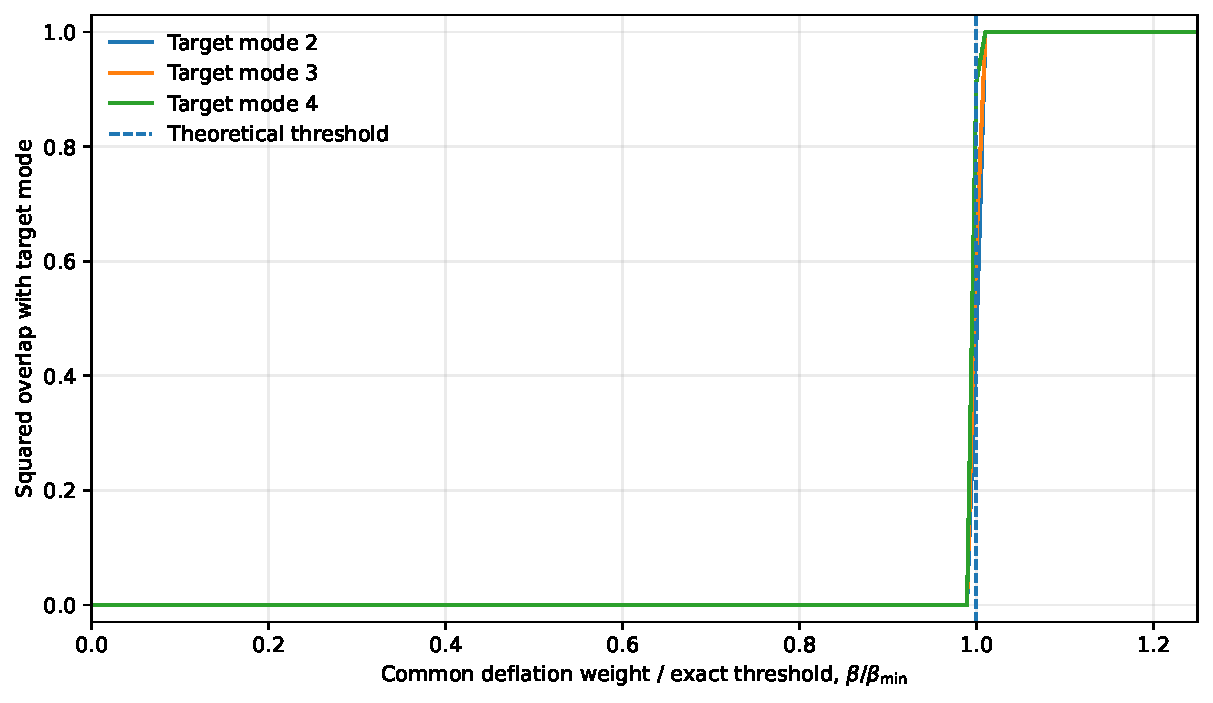
\includegraphics[width=\columnwidth]{penalty_threshold.pdf}
\caption{Exact deflation sweep for target modes 2--4. The target becomes the ground state only after the penalty exceeds the spectral threshold in \cref{eq:betathreshold}.}
\label{fig:penalty_threshold}
\end{figure}

Projector perturbations confirm the second half of the theory. With deflated separation $g_r=0.05$, projector rotation angles of 0.02, 0.04, and 0.06 rad produce target-state sine errors of 0.249, 0.413, and 0.508, while the conservative Davis--Kahan bounds are 0.273, 0.545, and 0.818. The bound is not tight, but correctly captures amplification by $\beta_j$ and loss of protection as $\norm{\Delta_r}$ approaches the separation.

\subsection{Gershgorin scaling is not the dominant problem in the tested chains}

The empirical Gershgorin ratio is shown in \cref{fig:gersh}. Across both mass models and $N=4$--128, the ratio lies between 1.014 and 1.110. Thus the bound is mildly conservative for these one-dimensional chains, although no universal tightness is claimed.

\begin{figure}[t]
\centering
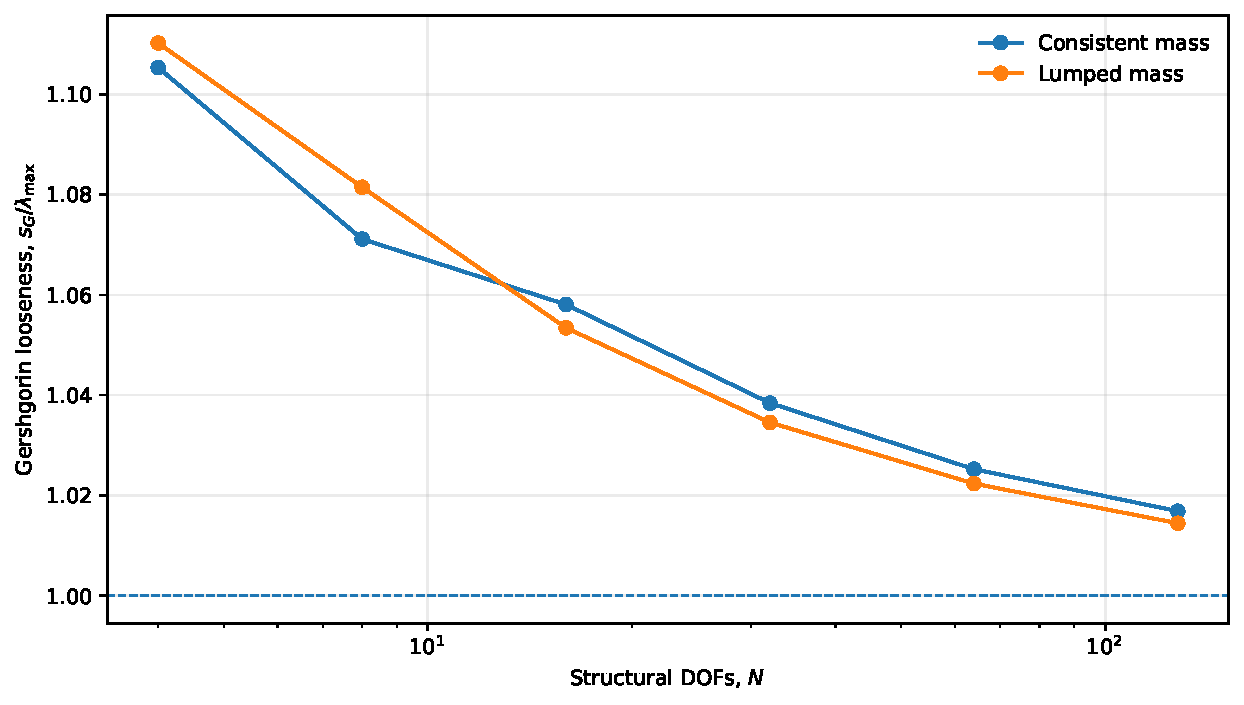
\includegraphics[width=\columnwidth]{gershgorin_tightness.pdf}
\caption{Gershgorin looseness for the structural-chain scaling study. The ratio approaches one with increasing $N$ for these particular models.}
\label{fig:gersh}
\end{figure}

The two-scale scheme remains useful because a different topology or material contrast can produce a looser bound, and because certified padding should not depend on the optimizer normalization.

\subsection{Mass whitening creates a measurable Pauli bottleneck}

\Cref{fig:density,fig:pauliscale} show the principal scaling result. At $N=128$, lumped mass yields transformed density 0.0233 and 576 nonzero Pauli terms; consistent mass yields density 0.3077 and 2950 terms. At $N=64$, greedy qubit-wise commuting groups increase from 64 for lumped mass to 221 for consistent mass.

\begin{figure}[t]
\centering
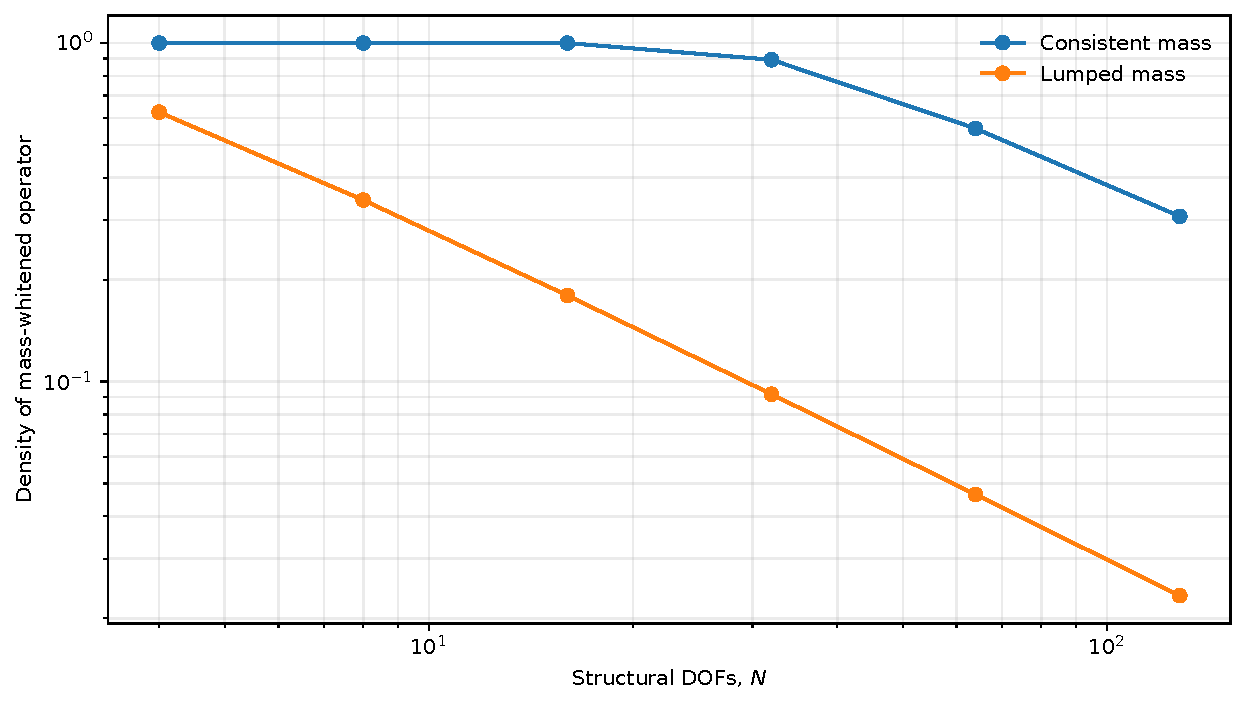
\includegraphics[width=\columnwidth]{whitening_density.pdf}
\caption{Density of the mass-whitened operator. Consistent mass introduces substantially more long-range coupling than lumped mass in the tested chains.}
\label{fig:density}
\end{figure}

\begin{figure}[t]
\centering
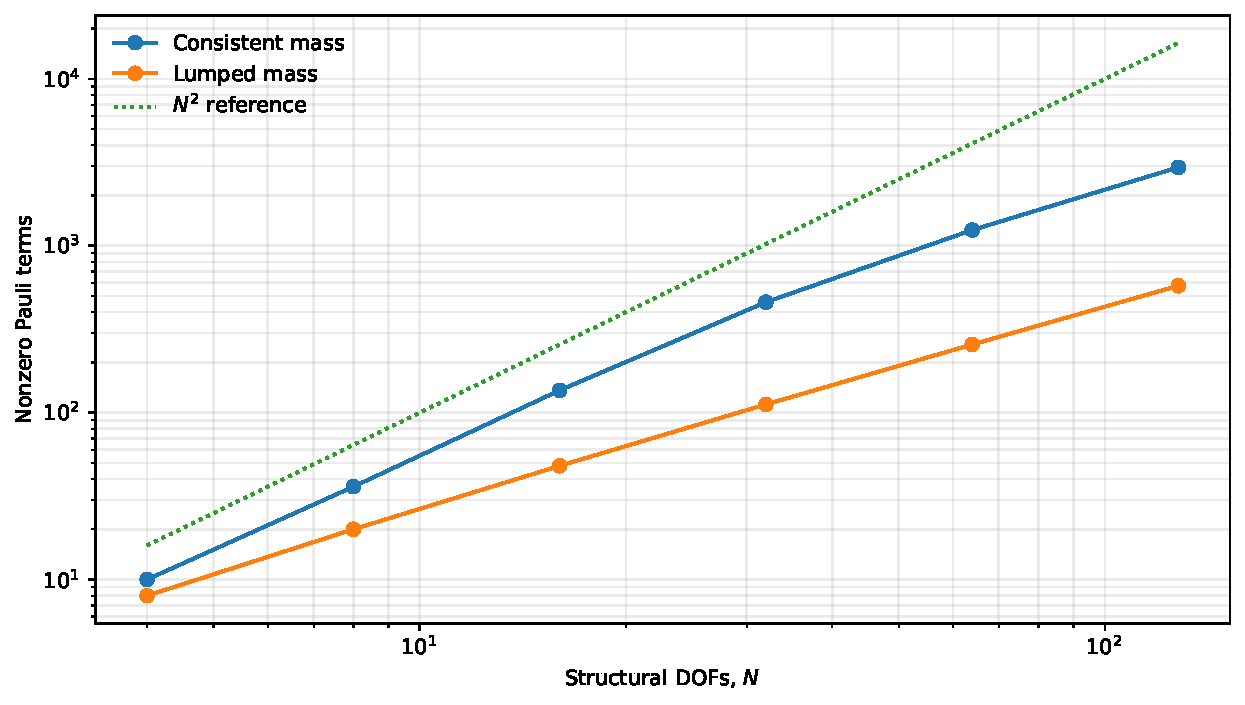
\includegraphics[width=\columnwidth]{pauli_scaling.pdf}
\caption{Nonzero Pauli-term count versus structural DOFs. The $N^2$ line is a reference, not a fitted asymptotic law.}
\label{fig:pauliscale}
\end{figure}

\begin{table}[t]
\centering
\caption{Selected Hamiltonian-scaling results. QWC denotes greedy qubit-wise commuting groups.}
\label{tab:scaling}
\begin{tabular}{lrrrrr}
\toprule
Mass & $N$ & $n_q$ & $s_G/\lambda_{\max}$ & Pauli terms & QWC groups\\
\midrule
Lumped & 16 & 4 & 1.053 & 48 & 16\\
Lumped & 64 & 6 & 1.022 & 256 & 64\\
Lumped & 128 & 7 & 1.014 & 576 & --\\
Consistent & 16 & 4 & 1.056 & 136 & 41\\
Consistent & 64 & 6 & 1.026 & 1241 & 221\\
Consistent & 128 & 7 & 1.017 & 2950 & --\\
\bottomrule
\end{tabular}
\end{table}

Preprocessing to $N=512$ confirms that the Cholesky factor of the chain remains banded, but $\A$ contains 1534 retained entries for lumped mass and 21554 for consistent mass. This is not evidence of universal dense scaling; it is direct evidence that whitening and mass formulation must be included in resource estimates.

\subsection{Circuit depth, not qubit count, controls exact-state recovery}

The 8- and 16-DOF fundamental-mode results are summarized in \cref{tab:vqe_depth} and \cref{fig:largervqe}. For 16 DOFs, depth 1 gives 81.75\% frequency error, depth 2 gives 5.16\%, and depth 3 gives $4.09\times10^{-9}$\%. The exact-state result shows that four qubits are enough to store the vector but not that a shallow circuit can prepare it.

\begin{table}[t]
\centering
\caption{State-vector VQE depth study for the fundamental mode.}
\label{tab:vqe_depth}
\begin{tabular}{rrrrr}
\toprule
$N$ & Qubits & Depth & Parameters & Frequency error (\%)\\
\midrule
8 & 3 & 1 & 6 & 27.33\\
8 & 3 & 2 & 9 & $5.22\times10^{-13}$\\
8 & 3 & 3 & 12 & $1.06\times10^{-12}$\\
16 & 4 & 1 & 8 & 81.75\\
16 & 4 & 2 & 12 & 5.16\\
16 & 4 & 3 & 16 & $4.09\times10^{-9}$\\
\bottomrule
\end{tabular}
\end{table}

\begin{figure}[t]
\centering
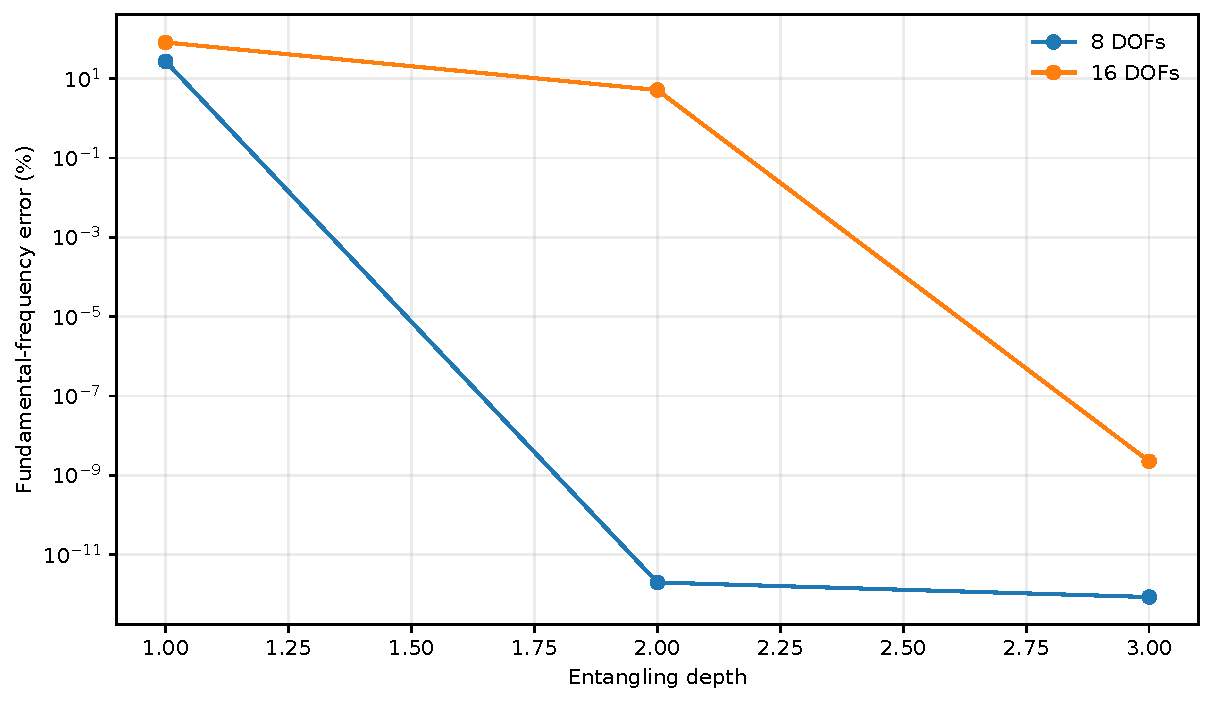
\includegraphics[width=\columnwidth]{larger_vqe_error.pdf}
\caption{Fundamental-frequency error versus circuit depth for 8- and 16-DOF chain models.}
\label{fig:largervqe}
\end{figure}

Twenty six-DOF restarts reinforce this interpretation. Depth 1 has a minimum first-mode error of 127.99\%, a median of 130.20\%, and a maximum of 130.20\%; depth 2 has a median error $4.3\times10^{-12}$\%. The shallow failure is therefore systematic ansatz error, not an unlucky optimizer seed.

\begin{remark}[Parameter-count lower bound on required depth]
The depth dependence in \cref{tab:vqe_depth} follows from a parameter count. A real, normalized state in $D=2^{n_q}$ dimensions has $D-1$ free amplitudes, whereas the real-amplitude circuit of \cref{eq:ansatz} at depth $L$ has $n_q(L+1)$ parameters. Reaching an arbitrary target therefore requires
\begin{equation}
n_q(L+1)\ge 2^{n_q}-1,
\qquad\text{equivalently}\qquad
L\ge\frac{2^{n_q}-1}{n_q}-1.
\label{eq:depthbound}
\end{equation}
This necessary condition predicts every row of \cref{tab:vqe_depth}: for $n_q=3$ it holds at $L=2$ ($9\ge7$) but not $L=1$ ($6<7$); for $n_q=4$ it holds at $L=3$ ($16\ge15$) but not $L=2$ ($12<15$). Since $2^{n_q}=N$, the required depth grows as $L=\Omega(N/\log_2 N)$, so a fixed-depth family cannot remain expressive as $N$ increases and the logarithmic qubit count does not translate into a logarithmic-depth circuit. The condition is necessary but not sufficient: the CNOT-ring entangler can further restrict the reachable manifold, so \cref{eq:depthbound} is a lower bound on the depth an exact preparation requires. This is consistent with the systematic shallow-circuit failure reported above.
\end{remark}

\subsection{Gradient statistics raise, but do not settle, the barren-plateau question}

\Cref{fig:gradients} reports gradient variance for a depth-2 circuit over 2--12 qubits, with bootstrap 95\% confidence intervals from the 80 samples per point. Under uniform initialization the variance declines from $2.62\times10^{-2}$ at 2 qubits to $9.82\times10^{-4}$ at 12 qubits. A power law in $n_q$ fits the uniform-initialization series better than an exponential: over the full range $R^2=0.96$ versus $0.83$, favouring the power law by $\Delta\mathrm{AIC}=15$; over the small-system-free range $n_q\ge4$ the advantage narrows to $R^2=0.90$ versus $0.85$ ($\Delta\mathrm{AIC}=4$, moderate). The decline does not stop: a linear fit to the tail ($n_q\ge7$) gives a shallow slope of $-0.12$ per qubit (95\% CI $[-0.23,-0.01]$), statistically nonzero but far below the per-qubit exponential rate that defines a barren plateau. Near-identity initialization produces smaller and nonmonotonic values, including $1.52\times10^{-5}$ at 12 qubits. Thus over the accessible range the gradients shrink at an approximately polynomial, not exponential, rate; $n_q\le12$ remains far from asymptotic, so the manuscript does not claim the definitive absence of a true barren plateau at larger scale.

\begin{figure}[t]
\centering
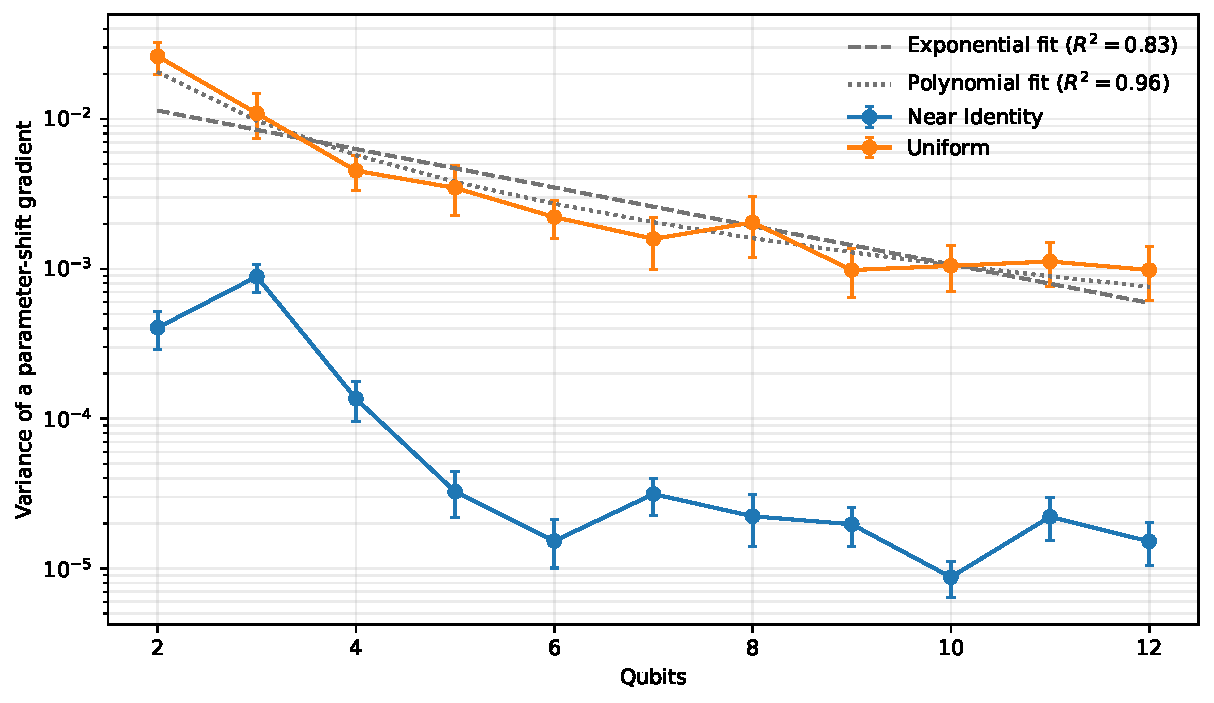
\includegraphics[width=\columnwidth]{gradient_trainability.pdf}
\caption{Empirical gradient variance for depth-2 real-amplitude circuits over 2--12 qubits, with bootstrap 95\% confidence intervals and polynomial and exponential fits to the uniform-initialization series. The variance is better fit by a power law than an exponential; the finite range is a diagnostic, not an asymptotic barren-plateau proof.}
\label{fig:gradients}
\end{figure}

\subsection{Finite-shot frequency estimation is most difficult for the first mode}

\Cref{fig:shotfreq,tab:shotfreq} show the independent-Pauli Monte Carlo results. At $10^4$ shots per Pauli term, frequency RMSE is 7.87\% for mode 1 but only 0.26\% for mode 4. Even at $10^5$ shots per term, mode-1 RMSE is 2.23\%. This follows from \cref{eq:freqvar}: the square-root transformation amplifies eigenvalue uncertainty at small $f_i$.

\begin{figure}[t]
\centering
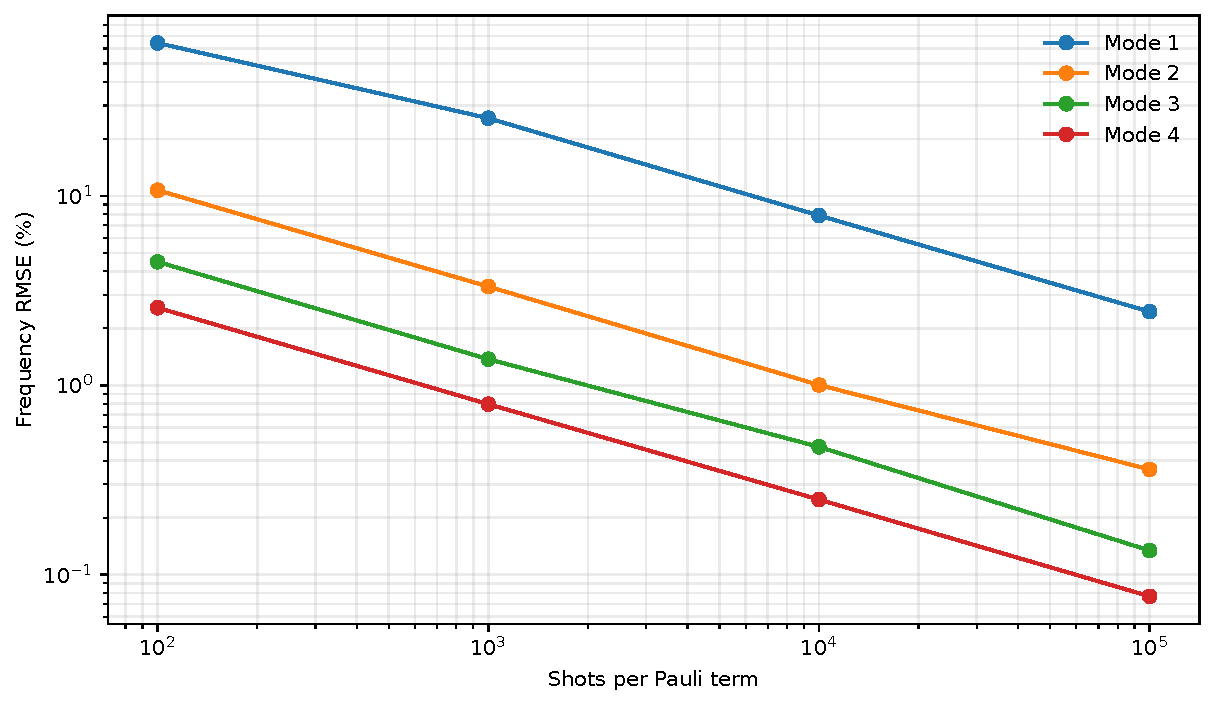
\includegraphics[width=\columnwidth]{finite_shot_frequency.pdf}
\caption{Finite-shot frequency RMSE from independent Pauli measurements of exact modal states.}
\label{fig:shotfreq}
\end{figure}

\begin{table*}[t]
\centering
\caption{Frequency RMSE (\%) under independent Pauli sampling and an optimistic QWC lower bound.}
\label{tab:shotfreq}
\begin{tabular}{lrrrr}
\toprule
Measurement budget & Mode 1 & Mode 2 & Mode 3 & Mode 4\\
\midrule
$10^2$ shots/term, independent & 64.11 & 10.78 & 4.72 & 2.47\\
$10^3$ shots/term, independent & 26.39 & 3.14 & 1.44 & 0.83\\
$10^4$ shots/term, independent & 7.87 & 1.03 & 0.45 & 0.26\\
$10^5$ shots/term, independent & 2.23 & 0.34 & 0.15 & 0.08\\
\midrule
QWC-optimal floor at matched total budget$^{\dagger}$ & 0.83 & 0.14 & 0.054 & 0.032\\
\bottomrule
\end{tabular}

\vspace{0.35em}
\parbox{0.97\textwidth}{\footnotesize $^{\dagger}$The six-DOF Hamiltonian has 19 nonidentity Pauli terms and eight greedy qubit-wise-commuting groups. The floor uses the same $1.9\times10^6$ total shots per mode as the $10^5$-shots-per-term baseline, exact within-group covariances, continuous optimal allocation, perfect simultaneous measurement, and no circuit, readout, or allocation overhead. It is therefore an optimistic lower bound, not an expected hardware result.}
\end{table*}

The independent experiment is a baseline, not an optimized measurement strategy. At matched total state preparations, exact-covariance QWC grouping lowers the theoretical RMSE floor by factors of approximately 2.5--2.8, but the first-mode floor remains 0.83\%. Thus grouping is valuable yet does not remove the low-frequency sensitivity. Classical shadows, hardware-efficient entangled measurements, and error mitigation should be compared in future work.

\subsection{Exact modal damage agreement does not survive finite sampling}

Exact-state agreement of the modal energy fractions with the classical solution is a consistency check only. The finite-shot localization study is more informative. \Cref{fig:shotdamage} shows that a 10\% stiffness loss is localized correctly in 26\% of 200 trials at $10^5$ shots per Pauli term (Wilson 95\% interval approximately 20.4--32.5\%), compared with a 16.7\% random baseline. A 20\% loss reaches 36\% (approximately 29.7--42.9\%). The median localization margin remains negative, meaning that an incorrect element usually exceeds the damaged element's score.

\begin{figure}[t]
\centering
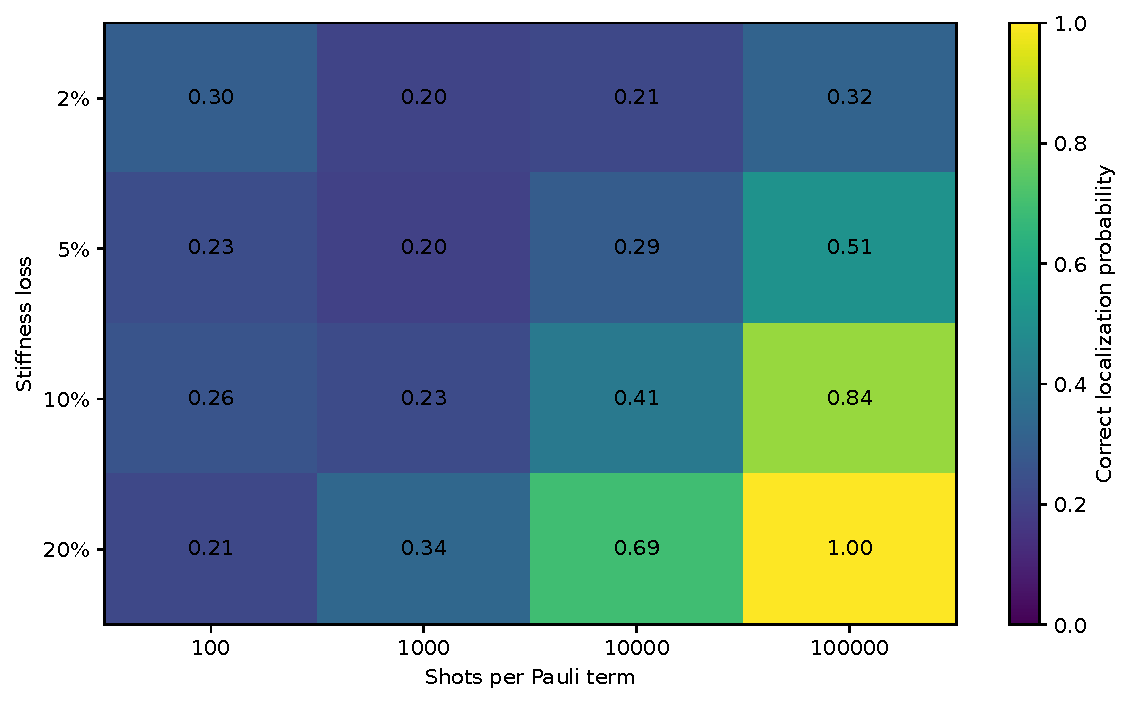
\includegraphics[width=\columnwidth]{damage_shot_localization.pdf}
\caption{Correct damage-localization probability from independently sampled element-energy observables. The random-guess baseline is $1/6=16.7\%$.}
\label{fig:shotdamage}
\end{figure}

This negative result independently tests the damage formulation and identifies measurement variance as a limiting factor. It does not invalidate modal strain energy as a classical SHM feature; it shows that direct independent-Pauli estimation is presently inefficient for small stiffness changes.

\section{Generalization to two and three dimensions}
\label{sec:dimensions}

Every experiment above uses a one-dimensional chain, the most favorable case for Cholesky fill. This section tests whether the mapping and deflation theory carry over unchanged to higher spatial dimension, and whether the densification finding of \cref{sec:mapping,sec:resources} is a property of the 1D chain specifically or worsens as dimension increases.

\subsection{What remains dimension-agnostic}

Nothing in the theory assumes a specific spatial dimension. The Cholesky mapping and mass--Euclidean isometry (Proposition~1) hold for any $\M\succ0$, $\K=\K^T$. Spectral-safe padding (Proposition~2) and the scalar-scaling law (Proposition~3) depend only on the spectrum of $\A$. The exact deflation theorem and the Davis--Kahan perturbation bound (Theorem~1, \cref{eq:dkbound}) hold for any Hermitian operator with a spectral gap, independent of what physical system it was built from. The parameter-count depth bound (Remark~2, \cref{eq:depthbound}) depends only on $n_q$, not on how the DOFs are arranged in space. The resource vector \cref{eq:resourcevector} and the finite-shot propagation formulas (\cref{eq:paulivar,eq:energyvar,eq:freqvar}) are likewise generic to any Pauli-decomposed Hamiltonian. Only the \emph{values} taken by $N_P$, the transformed density, and the Gershgorin ratio are specific to a given mesh, and those are what this section measures.

\subsection{Two- and three-dimensional scaling}
\label{sec:dim-scaling}

\begin{table*}[t]
\centering
\caption{Two- and three-dimensional scalar-mesh scaling, generalizing \cref{tab:scaling}. Grid sizes are chosen as exact powers of two, as in the 1D study.}
\label{tab:dimscaling}
\begin{tabular}{llrrrr}
\toprule
Dimension & Mass & $N$ & $n_q$ & Density of $\A$ & Pauli terms\\
\midrule
2D & Lumped & 16 & 4 & 0.250 & 48\\
2D & Lumped & 64 & 6 & 0.070 & 256\\
2D & Lumped & 256 & 8 & 0.019 & 1280\\
2D & Lumped & 1024 & 10 & 0.005 & 6144\\
2D & Consistent & 16 & 4 & 1.000 & 136\\
2D & Consistent & 64 & 6 & 1.000 & 2079\\
2D & Consistent & 256 & 8 & 0.947 & 25082\\
2D & Consistent & 1024 & 10 & 0.433 & 147620\\
3D & Lumped & 64 & 6 & 0.086 & 256\\
3D & Lumped & 128 & 7 & 0.045 & 576\\
3D & Lumped & 1024 & 10 & 0.006 & 6144\\
3D & Consistent & 64 & 6 & 1.000 & 2080\\
3D & Consistent & 128 & 7 & 1.000 & 8251\\
3D & Consistent & 1024 & 10 & 0.908 & 312325\\
\bottomrule
\end{tabular}
\end{table*}

The mesh is a scalar grid of point masses connected by nearest-neighbor springs, the direct $d$-dimensional generalization of the 1D chain: the same two-node element pattern is applied along $d$ axes instead of one, with one DOF per node so that the comparison isolates spatial dimension rather than DOFs per node. Free-DOF counts are fixed at exact powers of two by fixing an entire boundary layer along one axis, generalizing the chain's fixed base. Stiffness and mass vary smoothly and asymmetrically across the grid axes, exactly as the 1D study varies properties along the chain, so that no accidental grid symmetry inflates or deflates the sparsity count. \Cref{tab:dimscaling,fig:dimscaling} report density and nonzero Pauli terms for lumped and consistent mass at matched qubit counts.

\begin{figure}[t]
\centering
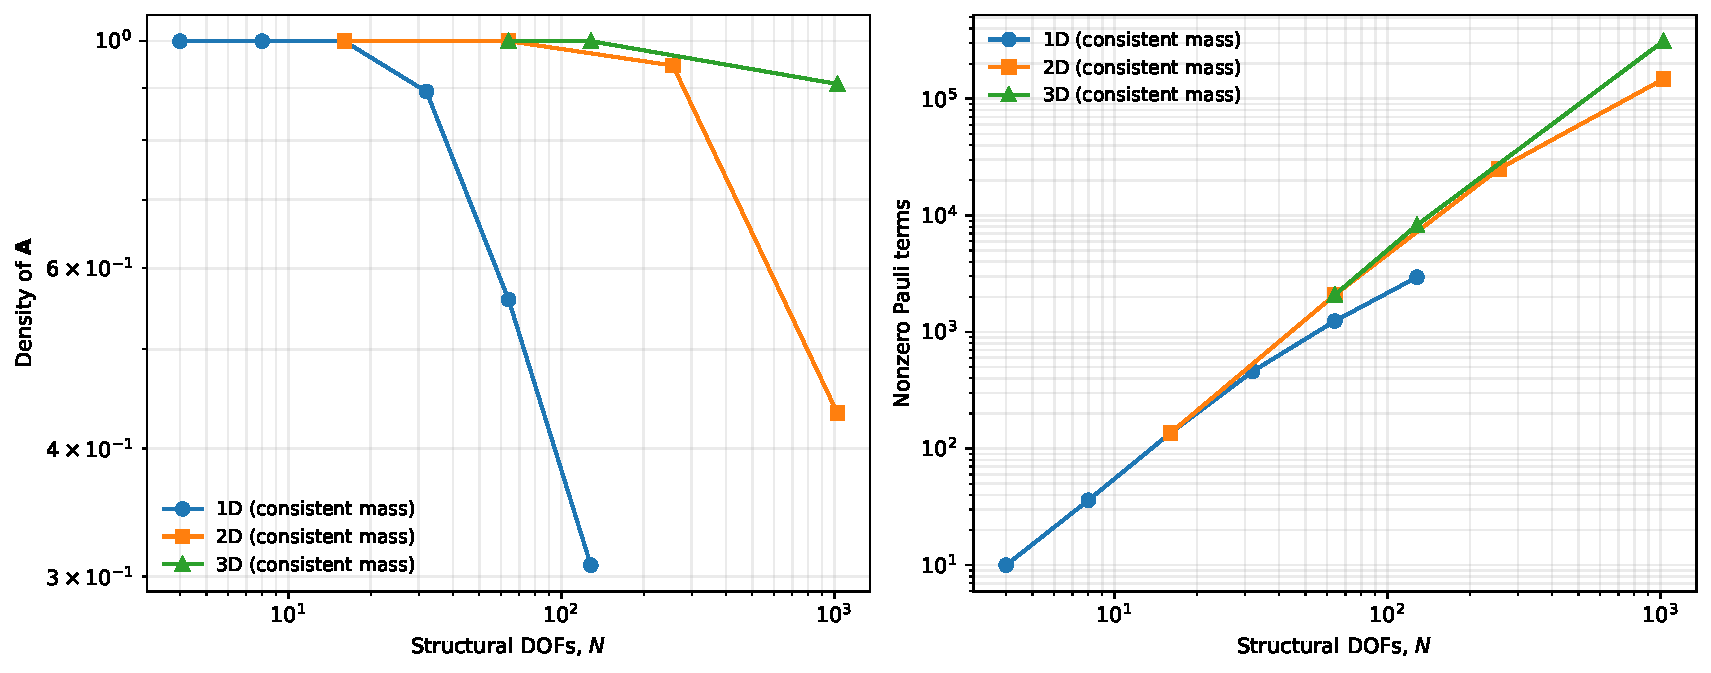
\includegraphics[width=\columnwidth]{dimension_scaling.pdf}
\caption{Transformed-operator density and nonzero Pauli-term count for consistent mass, 1D chains versus the 2D and 3D grids of \cref{tab:dimscaling}. The density-decline onset shifts to larger $N$ as dimension increases: 1D declines by $N\!\approx\!32$--64, 2D not until $N\!=\!1024$, and 3D remains 91\% dense at the largest tested size.}
\label{fig:dimscaling}
\end{figure}

Lumped mass remains markedly sparser than consistent mass at every tested size in every dimension, as in the 1D case. For consistent mass, the informative comparison is at matched $N$: at $N=1024$, 2D density has fallen to 0.433 while 3D remains at 0.908---the same DOF count, a visibly different regime. This is consistent with nested-dissection theory: 2D separator fill scales as $O(\sqrt N)$ and 3D as $O(N^{2/3})$ \cite{GeorgeNg1988}, so the onset of sparsity-recovering behavior is expected to shift to larger $N$ as dimension increases, and 3D should lag furthest behind. Fitting a single power law to the full tested range gives an increasing but modest exponent (1D $\approx\!1.66$, 2D $\approx\!1.69$, 3D $\approx\!1.79$); because density has not yet stabilized into a clean power-law regime in any dimension over the tested sizes, these exponents are reported as illustrative fits, not asymptotic laws, exactly as \cref{sec:results} already cautions for the 1D case. The Gershgorin ratio remains mild in every case tested (1.04--1.14), consistent with the 1D finding of \cref{fig:gersh} that Gershgorin looseness is not the dominant issue.

Declining density is a fractional effect: the absolute nonzero Pauli-term count continues to grow in every dimension tested (\cref{tab:dimscaling}), so this does not indicate that the measurement burden diminishes with $N$. The practical relevance of eventual sparsity recovery is also limited by scale. For an idealized cubic mesh, the graph diameter (maximum node-to-node hop distance) is $d(N^{1/d}-1)$ in $d$ dimensions; matching the diameter of the $N=128$ 1D chain already tested (127 hops) would require an idealized square mesh of $N\approx4{,}160$ (12 qubits) or an idealized cubic mesh of $N\approx81{,}000$ (16.3 qubits). This is an illustrative order-of-magnitude estimate for a regular cubic mesh, not a claim about arbitrary geometries, but it places any such recovery for 3D structures far beyond near-term hardware and, likely, beyond the regime in which classical simulation of the whitened operator itself remains convenient.

These results do not extend to irregular topology, block DOFs, or realistic 3D frames; they show that the 1D densification finding is not an artifact of one spatial dimension, and that it does not improve---if anything it worsens and appears later---as dimension increases.

\subsection{Validating the degeneracy diagnostics}
\label{sec:dim-degeneracy}

A 1D chain with smoothly varying properties has no repeated eigenvalues and so can never exercise the subspace-based diagnostic of \cref{eq:subspace}. A symmetric two-dimensional grid can: reflecting the grid across its diagonal is an exact symmetry, so a uniform square grid has genuinely degenerate mode pairs. Using a uniform (not the heterogeneous) grid from \cref{sec:dim-scaling}, an adjacent-eigenvalue pair was found with relative gap $2.2\times10^{-16}$, i.e.\ degenerate to floating-point precision.

For a degenerate pair, any rotation of the two eigenvectors within their shared subspace is an equally valid choice, so two independent solves (or a solver and a slightly perturbed rerun) may return differently oriented, but physically identical, bases. Let $\ph_a(\theta)=\cos\theta\,\ph_a+\sin\theta\,\ph_b$ be the pair rotated by angle $\theta$ within the degenerate subspace. Comparing $\ph_a$ to $\ph_a(\theta)$ via \cref{eq:mac} gives, since both are $\M$-orthonormal,
\begin{equation}
\MAC_{aa}^{(M)}(\theta)=\cos^2\theta,
\label{eq:macrotation}
\end{equation}
exactly---confirmed numerically to machine precision. \Cref{fig:degeneracy} shows this degrading from $1$ to $0.5$ at $\theta=45^\circ$ to essentially $0$ at $\theta=90^\circ$, which by conventional MAC thresholds would be flagged as a severe mismatch, even though the physical subspace never changed. The subspace-angle diagnostic \cref{eq:subspace} is stated in the whitened representation, where the isometry of Proposition~1 makes a plain transpose product equivalent to an $\M$-weighted one; written directly in the physical representation, it evaluates $\varepsilon_{\mathrm{sub}}$ between $\mathrm{span}(\ph_a,\ph_b)$ and its rotated copy via $(\mathbf Y_C)^T\M\mathbf Y_Q$. Since the rotation is an isometry of the shared subspace, this overlap matrix is exactly a $2\times2$ rotation matrix, whose singular values are exactly one, giving $\varepsilon_{\mathrm{sub}}=0$ for every $\theta$. The measured values stay at the eigensolver's numerical floor ($\sim\!3\times10^{-8}$) across the full sweep.

\begin{figure}[t]
\centering
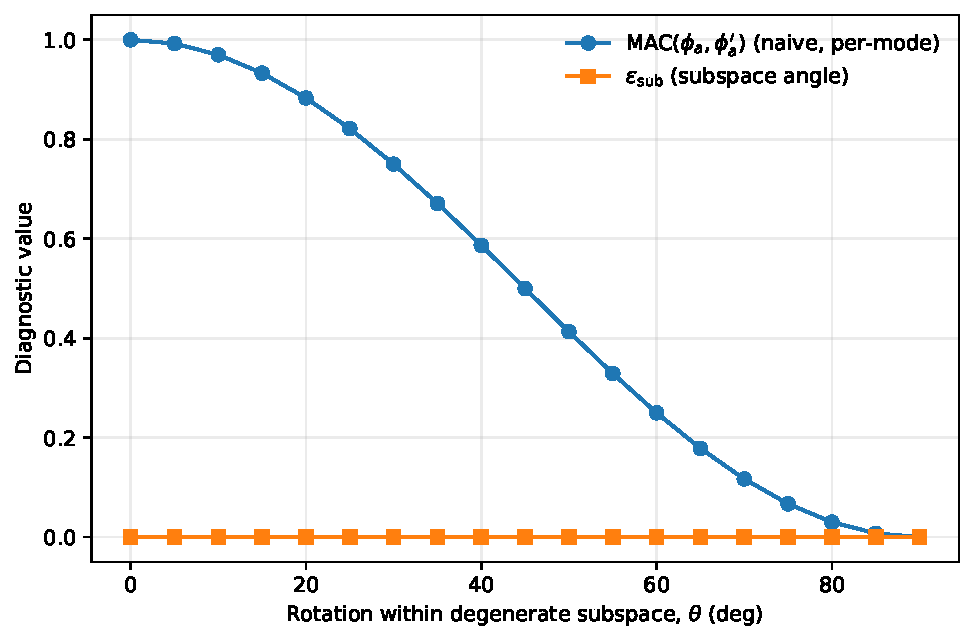
\includegraphics[width=\columnwidth]{degeneracy_demo.pdf}
\caption{Naive per-mode MAC versus the subspace-angle diagnostic for a genuine degenerate pair, rotated within its own subspace. MAC degrades exactly as $\cos^2\theta$ despite no physical change; $\varepsilon_{\mathrm{sub}}$ correctly remains at the numerical floor throughout.}
\label{fig:degeneracy}
\end{figure}

This is a direct demonstration of why \cref{sec:observables}'s subspace comparison exists: a per-mode diagnostic can manufacture a false structural-health alarm from an arbitrary, physically meaningless basis choice whenever a structure has near-symmetric geometry, and the subspace-angle diagnostic is immune to exactly that failure mode by construction.

\section{Discussion}
\label{sec:discussion}

\subsection{What is now theoretically guaranteed}

Three properties have exact statements. First, Cholesky whitening preserves eigenvalues and converts mass orthogonality to Euclidean orthogonality. Second, safe padding places artificial states above a certified physical bound for any positive optimization scale. Third, exact deflation identifies mode $r$ if and only if every lower-mode penalty exceeds its spectral difference from the target. With approximate prior states, \cref{eq:deflperturb,eq:dkbound} quantify the resulting loss of accuracy.

No theorem is claimed for global convergence of the parameterized circuit optimizer. This distinction is essential: a correct deflated operator can still be inaccessible to a shallow ansatz or missed by a nonconvex optimizer.

\subsection{Why heuristic composite penalties are unsafe}

A weighted cost $E+\gamma\sigma_H^2+\zeta\ell_p$ changes the optimization landscape without a universal conversion between energy, residual, and leakage. An adaptive multiplicative $\beta$ rule can overshoot the minimum spectral threshold and amplify projector error. Temporal overlap and frequency penalties can suppress genuine damage-induced changes. A scalar exponential integrity score can conceal a severe failure in one component behind good performance in another. Finally, a mixed-dimension ``information efficiency'' is uninterpretable without a reference task and cost model.

The proposed framework therefore uses theorem-based penalties, constrained diagnostics, independent epoch solutions, non-aggregated validation vectors, and raw resource counts.

\subsection{The actual scaling bottleneck}

For the tested chain models, Gershgorin looseness is modest. The more serious issue is that consistent-mass whitening changes operator structure, increasing nonzero Pauli terms and measurement groups; \cref{sec:dimensions} shows this bottleneck does not ease, and its onset shifts to larger $N$, as spatial dimension increases. The density of $\A$ is not an independent design variable: for fixed $\K$ and DOF ordering it is a deterministic consequence of the mass model through the Cholesky factor. The design tension is therefore a two-term causal chain rather than a trilemma,
\begin{equation}
\boxed{
\begin{aligned}
&\text{physical fidelity of }\M\\
&\quad\xrightarrow{\text{Cholesky}}\text{density of }\A\\
&\quad\xrightarrow{\text{Pauli}}\text{measurement cost}.
\end{aligned}}
\label{eq:trilemma}
\end{equation}
in which only the physical fidelity of $\M$ and the resulting measurement cost are genuinely in opposition; the intermediate density of $\A$ is induced, and is further modulated by DOF ordering and coefficient thresholding. Lumped mass may be cheaper quantum mechanically but can perturb high modes; consistent mass may be more faithful but measurement-heavy. A credible study must report both modal discretization error and quantum resource consequences.

As an illustration, consider the $N=128$, $k=4$ consistent-mass chain of \cref{tab:scaling}. \Cref{tab:concrete} contrasts the two routes with order-of-magnitude figures.

\begin{table}[t]
\centering
\caption{Illustrative end-to-end comparison for the $N=128$, $k=4$ consistent-mass chain. Preprocessing is finite-element assembly (classical) versus Cholesky factorization, whitening, and Pauli decomposition (quantum). Quantum figures are order-of-magnitude estimates, not measured device results.}
\label{tab:concrete}
\begin{tabular}{lll}
\toprule
Quantity & Classical & Quantum\\
\midrule
Qubits & --- & 7\\
Preprocessing & $O(N)$ & $O(N^2\log N)$\\
Nonzero Pauli terms & --- & 2950\\
Core work & ${\sim}1400$ matvecs & ${\sim}10^{11}$ circuits$^{\ddagger}$\\
Wall time & ${<}1$\,s & ${\sim}10^{5}$\,s\\
\bottomrule
\end{tabular}

\vspace{0.35em}
\parbox{\columnwidth}{\footnotesize $^{\ddagger}$${\sim}10^{5}$ shots per term $\times\,2950$ terms $\times$ a few hundred optimizer evaluations $\times\,4$ modes; the wall time assumes an optimistic $1\,\mu$s per circuit execution with no queueing, calibration, or readout overhead.}
\end{table}

The gap spans several orders of magnitude and is dominated by measurement, not preprocessing, which supports the qualitative statement that classical methods are overwhelmingly preferable for the present benchmarks. Any regime in which a quantum route could become competitive lies outside the variational setting studied here: it would require either fault-tolerant quantum phase estimation rather than sampling-based VQE, or operators that are genuinely dense so that classical sparsity offers no advantage---neither of which applies to sparse structural finite-element models. This is stated only to delimit scope and is not a claim of attainable advantage.

\subsection{Implications for structural health monitoring}

The finite-shot damage result changes the interpretation of quantum modal strain energy. The expectation-value identity is mathematically valid, but it is not automatically practical. Detection requires resolving a small difference between two noisy ratios of expectation values. For baseline and damaged estimates $\widehat a_d/\widehat b_d$ and $\widehat a_0/\widehat b_0$, a first-order variance is
\begin{equation}
\begin{aligned}
\Var(\widehat\eta_d-\widehat\eta_0)
&\approx \mathbf g_d^T\boldsymbol\Sigma_d\mathbf g_d
+\mathbf g_0^T\boldsymbol\Sigma_0\mathbf g_0,\\
\mathbf g&=\begin{bmatrix}1/b&-a/b^2\end{bmatrix}^T.
\end{aligned}
\label{eq:ratiovar}
\end{equation}
For equal shots $n$ per nonidentity Pauli term, write $\Var(\widehat D_e)\approx V_{D,e}/n$. A normal-approximation design criterion for detecting a nonzero score at two-sided type-I error $\alpha$ and power $1-\beta$ is
\begin{equation}
\boxed{
n_{\mathrm{det}}\gtrsim
\frac{(z_{1-\alpha/2}+z_{1-\beta})^2V_{D,e^\star}}
{D_{e^\star}^2}.
}
\label{eq:shotsdetect}
\end{equation}
For localization, let $e^{(2)}$ be the strongest intact competitor and $\Delta_D=D_{e^\star}-D_{e^{(2)}}$. A conservative Bonferroni pairwise requirement is
\begin{equation}
\boxed{
n_{\mathrm{loc}}\gtrsim
\frac{(z_{1-\alpha/(n_e-1)}+z_{1-\beta})^2V_{\Delta_D}}
{\Delta_D^2},
}
\label{eq:shotslocalize}
\end{equation}
where $V_{\Delta_D}$ is the per-shot variance coefficient of the score margin. The absolute-value signs are linearized at their exact signs. These expressions are design approximations, not finite-sample guarantees.

\begin{table*}[t]
\centering
\caption{Delta-method shots per Pauli term for the six-DOF damage example ($\alpha=0.05$, 80\% power).}
\label{tab:shotrequirements}
\begin{tabular}{rrr}
\toprule
Stiffness loss & Detect damaged-element change & Localize against all five competitors\\
\midrule
2\%  & $1.32\times10^7$ & $1.27\times10^9$\\
5\%  & $2.04\times10^6$ & $2.11\times10^8$\\
10\% & $4.82\times10^5$ & $5.71\times10^7$\\
20\% & $1.10\times10^5$ & $1.83\times10^7$\\
\bottomrule
\end{tabular}
\end{table*}

The calculation uses the first four modes with equal weights, independent baseline/damaged numerator and denominator estimates, and independent element-score variances. It is conservative because beneficial shared-denominator covariance is ignored. For 10\% damage, $10^5$ shots per term give a localization signal-to-noise ratio of only 0.13, consistent with the observed 26\% success being only modestly above random guessing. Approximately $4.8\times10^5$ shots per term are required to detect the damaged-element score with 80\% power, whereas reliable family-wise localization requires roughly $5.7\times10^7$ per term. With 648 nonidentity operator-term settings across four modes, six elements, and two structural states, the latter corresponds to approximately $3.7\times10^{10}$ circuit shots under the independent baseline. This suggests that covariance-aware joint measurement and direct estimation of change observables are not optional refinements but central algorithmic requirements.

\subsection{End-to-end quantum advantage remains unestablished}

Any future advantage claim must include:
\begin{enumerate}[label=(\alph*)]
\item assembly and reduction of $\M$ and $\K$;
\item factorization or generalized-quotient preparation;
\item Hamiltonian construction and Pauli decomposition;
\item state preparation and repeated measurements;
\item optimizer evaluations and higher-mode deflation;
\item readout of decision-relevant structural observables;
\item comparison with sparse classical eigensolvers at matched accuracy.
\end{enumerate}
For the present benchmarks, classical methods are overwhelmingly preferable.

\section{Limitations and research agenda}
\label{sec:limitations}

The main structural models remain one-dimensional chains, the most favorable case for Cholesky fill; \cref{sec:dimensions} reports an initial two- and three-dimensional scalar-mesh generalization confirming that densification does not improve, and appears later in $N$, as dimension increases. That study nonetheless uses regular scalar grids, not the block DOFs, irregular topology, constraints, and material heterogeneity of real bridges and buildings, and the measured exponents must not be extrapolated to such structures or to alternative DOF orderings and block-sparse formulations. Pauli decomposition is evaluated only under binary amplitude encoding. The finite-shot study uses independent Pauli measurements and exact input states; it does not include circuit noise, state-preparation error, grouped covariance, or device calibration. The damage study uses stiffness-only damage and no environmental variability. Cholesky timings are platform-specific, while the structural sparsity counts are more portable.

The next high-impact study should combine:
\begin{enumerate}[label=(\roman*)]
\item a laboratory frame or bridge dataset with FDD/SSI uncertainty;
\item block-sparse three-dimensional finite elements and alternative DOF orderings;
\item Cholesky, generalized quotient, and domain-decomposed mappings;
\item grouped or shadow-based measurement of modal observables;
\item near-degenerate subspace tracking under temperature and damage;
\item a matched end-to-end comparison against ARPACK/Lanczos and reduced-order classical models.
\end{enumerate}

\section{Conclusions}
\label{sec:conclusion}

This paper establishes a stricter evaluation standard for variational quantum modal analysis. The mass-orthonormal Cholesky map is physically consistent, but its preprocessing and densification costs are not negligible. Gershgorin bounds can certify padding without fixing the optimizer scale. Higher-mode penalties admit an exact threshold, and approximate-projector perturbation theory shows why oversized penalties are dangerous. Variance and leakage should be diagnostics or constrained refinements, not arbitrarily weighted additions to the primary energy. Temporal mode identity should be assigned after independent eigensolution so that continuity cannot mask damage.

The expanded experiments show both promise and difficulty. Increasing circuit depth recovers small exact-state modal problems, while a shallow ansatz fails systematically despite sufficient qubit dimension. In the tested chains, consistent mass substantially increases Hamiltonian density and Pauli count, and an initial two- and three-dimensional generalization shows this effect worsening, not improving, with spatial dimension, while also validating a subspace diagnostic on a genuine degenerate pair unavailable in one dimension. Finite-shot frequency and damage estimates remain costly, with the lowest mode particularly sensitive to sampling variance. These results do not establish quantum advantage. They identify the mathematical conditions and resource bottlenecks that a future structural quantum algorithm must overcome.

The main conclusion is therefore precise: qubits are necessary to encode the state, but spectrally valid modes, expressive circuits, sparse observables, and decision-level measurement precision are necessary to solve the engineering problem.

\section*{Data and code availability}
The accompanying archive contains the complete LaTeX source, bibliography, generated figures, CSV results, and Python scripts required to reproduce the exact-state, scaling, trainability, finite-shot, and damage-localization studies, together with the two- and three-dimensional generalization and degeneracy-diagnostic study of \cref{sec:dimensions}.

\section*{Conflict of Interest}
The author declares no conflict of interest.

% \section*{Acknowledgment}


\appendices
\section{Representative finite-element matrices}
For a two-dimensional truss element with $c=\cos\theta$ and $s=\sin\theta$,
\begin{equation}
\K_e=\frac{EA}{L}
\begin{bmatrix}
c^2&cs&-c^2&-cs\\
cs&s^2&-cs&-s^2\\
-c^2&-cs&c^2&cs\\
-cs&-s^2&cs&s^2
\end{bmatrix}.
\end{equation}
For an Euler--Bernoulli beam bending element,
\begin{equation}
\K_e=\frac{EI}{L^3}
\begin{bmatrix}
12&6L&-12&6L\\
6L&4L^2&-6L&2L^2\\
-12&-6L&12&-6L\\
6L&2L^2&-6L&4L^2
\end{bmatrix},
\end{equation}
\begin{equation}
\M_e=\frac{\rho AL}{420}
\begin{bmatrix}
156&22L&54&-13L\\
22L&4L^2&13L&-3L^2\\
54&13L&156&-22L\\
-13L&-3L^2&-22L&4L^2
\end{bmatrix}.
\end{equation}

\section{Sequential modal algorithm with provable deflation thresholds}
\begin{algorithm}[t]
\caption{Mass-orthonormal sequential VQE with provable deflation thresholds}
\label{alg:certvqe}
\begin{algorithmic}[1]
\Require Reduced $\M\succ0$, $\K=\K^T$; target modes $m$; ansatz family; tolerances.
\State Compute $\M=\mathbf L\mathbf L^T$ using a sparse ordering where appropriate.
\State Form $\A=\mathbf L^{-1}\K\mathbf L^{-T}$ by triangular solves.
\State Compute certified $U_G$ and choose optimization scale $s_t$.
\State Form $\Hq_p$ with $\alpha=U_G/s_t+\delta_p$.
\State Decompose the required operators and group compatible measurements.
\For{$r=1,\ldots,m$}
  \State Select and record the bound policy: $U_r=U_G/s_t$, or compute $U_r=\vartheta_r^{(p)}+\delta_{\mathrm{fp}}$ by a $p$-dimensional Ritz/Lanczos pass and record $C_{\mathrm{bound}}$.
  \For{$j<r$}
    \State Obtain $\delta_j$ from exact validation data or the declared residual-plus-shot confidence rule in \cref{eq:deltabound}.
    \State Set $\beta_j=U_r-\widehat\varepsilon_j+\delta_j+\tau$.
  \EndFor
  \State Minimize $C_r(\theta)=\langle\psi(\theta)|\widehat\Hq_r|\psi(\theta)\rangle$ over multiple initializations.
  \State Optionally solve the constrained variance refinement in \cref{eq:lexico}.
  \State Reject or flag the state if any component of \cref{eq:diagnosticvector} exceeds its declared tolerance.
  \State Recover $f_r$ and $\ph_r$ using \cref{eq:freqrecover,eq:recover}.
\EndFor
\end{algorithmic}
\end{algorithm}

For the reproducible six-DOF exact-state validation, the declared acceptance set was
\begin{equation}
\begin{aligned}
\epsilon_f&\le10^{-4}\%, &
\rho&\le10^{-5}, &
\sigma_H^2&\le10^{-10},\\
\ell_p&\le10^{-8}, &
o&\le10^{-8}, &
1-\MAC^{(M)}&\le10^{-6}.
\end{aligned}
\label{eq:exampletolerances}
\end{equation}
These values are numerical verification tolerances, not universal SHM thresholds. They accept all four depth-2 exact-state modes and reject the depth-1 results. Field applications must replace them with tolerances calibrated to model discrepancy, environmental variability, and decision consequences.

\section{Exact relation between projector error and state angle}
For normalized vectors $u$ and $\widehat u$, the rank-one projector difference satisfies
\begin{equation}
\norm{\widehat u\widehat u^T-uu^T}_2=\sin\angle(\widehat u,u).
\label{eq:projectorangle}
\end{equation}
Therefore the deflation perturbation may be written as
\begin{equation}
\norm{\Delta_r}_2\le
\sum_{j<r}\beta_j\sin\angle(\widehat u_j,u_j),
\label{eq:anglepert}
\end{equation}
which gives a direct rule for balancing penalty margin against the quality of previously extracted modes.


\bibliographystyle{IEEEtran}
\bibliography{references}

\EOD
\end{document}
